% \documentclass[acmsmall,screen,review]{acmart}
\documentclass[acmsmall,screen,review,anonymous]{acmart}
\citestyle{acmauthoryear}
\usepackage[utf8]{inputenc}
\usepackage[boxed,lined,linesnumbered]{algorithm2e}
\usepackage[english]{babel}
\usepackage[strings]{underscore}
\usepackage{amsthm, textcomp, gensymb, multirow, multicol, array, bm, float, setspace, paralist, subfig, enumitem, microtype, adjustbox, framed, xcolor, fix-cm}
\DeclareMathAlphabet{\mathcal}{OMS}{cmsy}{m}{n}
\graphicspath{{Figures/}}
%% ------------------------------------------------------------------
%% Nomenclature
\newcommand{\codecomm}[1]{\texttt{\small `#1'}}
\newcommand{\Pcl}{\mathcal{P}}
\newcommand{\Fcl}{\mathcal{F}}
\newcommand{\Acl}{\mathcal{A}}
\newcommand{\Scl}{\mathcal{S}}
\newcommand{\Ycl}{\mathcal{Y}}
\newcommand{\Rbb}{\mathbb{R}}
\newcommand{\Bin}{\mathbb{B}}
\newcommand{\A}{\mathbf{A}}
\newcommand{\B}{\mathbf{B}}
\newcommand{\Cbf}{\mathbf{C}}
\newcommand{\D}{\mathbf{D}}
\newcommand{\F}{\mathbf{F}}
\newcommand{\Ft}{\tilde{\F}}
\newcommand{\Ibf}{\mathbf{I}}
\newcommand{\Pbf}{\mathbf{P}}
\newcommand{\R}{\mathbf{R}}
\newcommand{\V}{\mathbf{V}}
\newcommand{\X}{\mathbf{X}}
\newcommand{\Y}{\mathbf{Y}}
\newcommand{\Z}{\mathbf{Z}}
\newcommand{\Xbar}{\overline{\X}}
\newcommand{\Ybin}{\Y_{\textrm{bin}}}
\newcommand{\Yhat}{\widehat{\Y}}
\newcommand{\f}{\mathbf{f}}
\newcommand{\p}{\mathbf{p}}
\newcommand{\vbf}{\mathbf{v}}
\newcommand{\y}{\mathbf{y}}
\newcommand{\z}{\mathbf{z}}
\newcommand{\frm}{\mathrm{f}}
\newcommand{\ybest}{\y^{*}}
\newcommand{\phat}{\hat{\p}}
\newcommand{\blambda}{\bm{\lambda}}
\newcommand{\bsigma}{\bm{\sigma}}
\newcommand{\biota}{\bm{\iota}}
\newcommand{\bmu}{\bm{\mu}}
\newcommand{\FALSE}{\textsc{FALSE}}
\newcommand{\TRUE}{\textsc{TRUE}}
\newcommand{\NaN}{\text{NaN}}
\newcommand{\flag}[1]{\phi_{\textrm{#1}}}

\setcopyright{acmlicensed}
\copyrightyear{2025}
\acmYear{2025}
\acmDOI{XXXXXXX.XXXXXXX}
\acmISBN{978-1-4503-XXXX-X/2018/06}

% ===================================================================
\begin{document}
% ===================================================================

\title{An Instance Space Analysis of Neural Network Training as a Black-Box Optimisation Problem}

\author{Katherine Mary Malan}
\email{malankm@unisa.ac.za}
\orcid{0000-0002-6070-2632}
\affiliation{%
    \institution{Department of Decision Sciences, University of South Africa}
    \city{Muckleneuk}
    \state{Pretoria}
    \country{South Africa}
}
 
\author{Mario Andrés Muñoz}
\email{munoz.m@unimelb.edu.au}
\orcid{0000-0002-7254-2808}
\affiliation{%
    \institution{School of Computing and Information Systems, The University of Melbourne}
    \city{Parkville}
    \state{VIC}
    \country{Australia}
}

\begin{CCSXML}
<ccs2012>
   <concept>
       <concept_id>10003752.10003809.10003716.10011138.10011803</concept_id>
       <concept_desc>Theory of computation~Bio-inspired optimization</concept_desc>
       <concept_significance>500</concept_significance>
       </concept>
   <concept>
       <concept_id>10010147.10010257.10010293.10010294</concept_id>
       <concept_desc>Computing methodologies~Neural networks</concept_desc>
       <concept_significance>500</concept_significance>
       </concept>
   <concept>
       <concept_id>10002944.10011123.10010912</concept_id>
       <concept_desc>General and reference~Empirical studies</concept_desc>
       <concept_significance>300</concept_significance>
       </concept>
   <concept>
       <concept_id>10002944.10011123.10011131</concept_id>
       <concept_desc>General and reference~Experimentation</concept_desc>
       <concept_significance>300</concept_significance>
       </concept>
   <concept>
       <concept_id>10002944.10011123.10011674</concept_id>
       <concept_desc>General and reference~Performance</concept_desc>
       <concept_significance>100</concept_significance>
       </concept>
 </ccs2012>
\end{CCSXML}

\ccsdesc[500]{Theory of computation~Bio-inspired optimization}
\ccsdesc[500]{Computing methodologies~Neural networks}
\ccsdesc[300]{General and reference~Empirical studies}
\ccsdesc[300]{General and reference~Experimentation}
\ccsdesc[100]{General and reference~Performance}

\begin{abstract}
        Training a neural network is an optimisation task that is commonly solved using gradient-based techniques, such as stochastic gradient descent or Adam. There are, however, scenarios in which black-box optimisation approaches, such as evolutionary algorithms, may be appropriate for optimising neural network weights. In this study, we view neural network weight optimisation as a black-box problem and analyse the search space using exploratory landscape analysis (ELA). The purpose is to understand what makes neural network search spaces different from other bound-constrained continuous-valued problems commonly used for benchmarking evolutionary algorithms. We perform an instance space analysis on a combined set of neural network training instances and instances from the widely used Black-Box Optimisation Benchmarking (BBOB) problem suite. The analysis included instances with 41, 261, and 481 decision variables, corresponding with 1-, 3-, and 5-layer networks. We show that neural-network training instances and BBOB instances occupy distinct regions of the ELA feature space. While the landscapes of BBOB instances typically exhibit strong global structure and large differences between local and global optima, neural network instances exhibit ill-conditioned landscapes with very weak global structure. Surprisingly, these instances were easier than BBOB instances for black-box algorithms to find acceptable solutions, likely due to the abundance of high-quality solutions. Another key and unexpected finding was that the features of the neural network error landscapes were more strongly influenced by the choice of activation function and the network size than by the underlying machine learning task, in this case the regression function to be fitted. 
\end{abstract}

\keywords{optimisation benchmarking, CORNN suite, exploratory landscape analysis, neural network training, instance space analysis}

\maketitle

% ===================================================================
\section{Introduction}

Neural networks, the basic machine learning model underlying most artificial intelligence (AI) systems in use today, rely on algorithms for training. This training is an optimisation task in which the network parameters (weights) are adjusted to minimise the error on a learning task. The most common algorithms for adjusting neural network weights exploit the gradient of the error function to guide the search. However, when gradient information is not readily available, alternative strategies such as evolutionary or swarm-based optimisation algorithms can be used. These approaches are ``black-box'' in nature, because the search is guided only by output errors on the learning task, with no additional information about the underlying function to be optimised.   

Over the last few decades, the development of black-box algorithms has benefited substantially from competitions with their associated benchmark problem sets, such as BBOB~\cite{BBOB} and CEC~\cite{CEC}. These competitions use functions expressed in mathematical form that are carefully chosen to capture a range of problem features, such as separability, modality, and conditioning level. However, neural network training tasks exhibit characteristics distinct from those of commonly used benchmark problems~\cite{Malan2025}. For example, benchmark functions typically have a single global optimum, while neural network landscapes are known to have multiple global optima due to the inherent symmetry in neural networks~\cite{BOSM2019Thesis}. To be used appropriately for neural network training, further work is needed to analyse the strengths and weaknesses of black-box algorithms on problems with these characteristics.

\citet{SmithMiles2014} proposed the instance space analysis (ISA) methodology in 2014, where the performance of different algorithms could be visualised and compared across a feature space of problem instances. This was a new approach to performance assessment that highlighted the strengths and weaknesses of algorithms across different groups of instances (distinguished by problem features), rather than the common practice of comparing algorithms based on average performance over the entire set of benchmark instances. The two main ways that ISA is commonly used are to:
\begin{inparaenum}[(a)]
    \item objectively test algorithms on a set of instances, and
    \item assess the diversity of a set of problem instances~\cite{SmithMiles2022}.
\end{inparaenum}

In the last few years, ISA has gained popularity as a tool for analysing a wide range of optimisation problems with candidate algorithms, including knapsack problems~\cite{SmithMiles2021}, clustering~\cite{Fernandes2021}, personnel scheduling~\cite{Kletzander2020}, regression problems~\cite{Munoz2021}, course timetabling~\cite{DeCoster2021}, constrained multiobjective problems~\cite{Alsouly2023}, and the optimisation of test scenarios for autonomous vehicles~\cite{CrespoRodriguez2025}. In this paper, we use ISA to analyse neural network training tasks as black-box optimisation problems. The purpose is to investigate how neural network optimisation differs from standard continuous optimisation benchmark instances and to better understand how black-box algorithms perform on these neural network instances.
%In previous work at the Genetic and Evolutionary Computation Conference (GECCO)~\cite{Malan2025} we presented results 

\citet{Malan2025} conducted a study comparing the search landscape features of 41-dimensional neural network training tasks with those of 41-dimensional BBOB functions. In this paper, we build on that work by extending the instances to higher-dimensional search spaces (261- and 481-dimensional). In addition, we conduct a full analysis of the instance space by including performance data of four black-box algorithms.

In summary, the main contributions of the paper are as follows:
\begin{enumerate}
    \item We conduct exploratory landscape analysis on neural network regression problem instances and BBOB instances in 41, 261, and 481 dimensions.
    \item We measure the performance of four black-box algorithms on the same problem instances.
    \item We conduct an instance space analysis of the problem instances to show that the features of neural network error landscapes differ from those of BBOB instances.
    \item To facilitate reproducibility and extension of the work, we share all code and data in public repositories.
\end{enumerate}

% ===================================================================
The rest of the paper is organised as follows. Section \ref{sec:Background} provides a summary of background concepts; Section~\ref{sec:instance_space} describes how ISA was implemented in this study; the results are presented in Section~\ref{sec:results} followed by conclusions in Section~\ref{sec:conclusion}. 

\section{Background}\label{sec:Background}
% ===================================================================
This section provides a summary of three background concepts related to this study:
\begin{inparaenum}[(a)]
    \item the training of neural networks as a black-box optimisation task, 
    \item the previously proposed CORNN suite of neural network regression tasks, and 
    \item exploratory landscape analysis for numerically characterising the features of optimisation problem instances.
\end{inparaenum}

% ===================================================================
\subsection{Optimising the weights of neural networks}\label{sec:NN_training}
% ===================================================================
To train a neural network, data are presented as input to the network, the output is calculated, and weights are then adjusted with the aim of minimising the error on some machine learning task. The most common approach to adjusting weights is to exploit gradient information of the error function with respect to the weights. These gradient-based techniques, such as stochastic gradient descent and Adam, are effective even for very large networks, due to the computational efficiency of component-wise updates based on predetermined analytical partial derivatives. 

If the $n$ trainable weights of a neural network are combined into a vector, then the resulting $n$-dimensional search space can be effectively optimised using population-based metaheuristics~\cite{MOUS2020,SOCH2007,VAND2000}. This approach to training neural networks would be regarded as ``black-box", because the algorithm is only guided using the error of the network as an objective function. A black-box alternative to a gradient-based approach could be effective in scenarios such as the following:

\begin{itemize}
    \item In environments where reinforcement learning is used to train agents, feedback is often sparse, and there can be a delay before agents receive rewards for their actions. In these data-scarce scenarios, gradient information is often unavailable, and algorithms that prioritise wider exploration may be more appropriate~\cite{Salimans2017, Conti2018}. 

    \item In scenarios where neural networks should have hard decision boundaries, activation functions such as the step function can be used. Since these functions are non-differentiable, black-box optimisation approaches are a viable alternative. 
  
    \item Product unit neural networks (PUNNs) are higher-order networks that differ from standard neural networks in that the net input signal is a weighted product of inputs, rather than a weighted sum. Black-box algorithms are more suitable for training PUNNs than gradient-based approaches due to the treacherous gradients evident in these loss landscapes~\cite{Engelbrecht2024}.
\end{itemize}

In this study, we provide insights into the nature of the search spaces in neural network training. The aim is to understand how these spaces differ from those of commonly used benchmark optimisation problems and to shed light on how different metaheuristics perform in different regions of the instance space.

% ===================================================================
\subsection{The CORNN suite}
% ===================================================================
\citet{Malan2022} proposed the CORNN suite of neural network regression training tasks to be used as a benchmark for continuous black-box algorithms. The suite comprises over 300 learning tasks involving the optimisation of weights of different neural network architectures and activation function combinations to approximate a range of two-dimensional functions. The 54 functions used in CORNN include functions commonly used as optimisation benchmarks, such as the Ackley function. However, in the context of CORNN, the functions are not optimised directly; instead, they are used as regression fitting tasks, and the optimisation task involves searching for the combination of neural network weights that best approximates the two-dimensional function. 

For each of the 54 2$D$ functions, a training dataset and a testing dataset are provided. The datasets were generated using a uniform random sample of 5~000 points from the domain of the function, randomly split into training (75\%) and test sets (25\%). The training set, therefore, consists of 3~750 $(x_1,x_2)$ pairs of input values (normalised to the range $[-1,1]$) with the associated target value (the true output of the function corresponding with the input pair), while the test set consists of the remaining 1~250 samples of input pairs and output targets. 

The CORNN suite comprises neural network architectures with one, three, and five layers, with each layer consisting of ten neurons and a bias unit. This results in optimisation instances with 41, 261, and 481 dimensions corresponding with the number of weights in the 1-, 3-, and 5-layer models. Two versions of each neural network model are provided using the hyperbolic tangent (Tanh) and rectified linear unit (ReLU) activation functions in the hidden layers. 

In the original CORNN suite study~\cite{Malan2022}, performance data were presented on four black-box optimisation algorithms: particle swarm optimisation (PSO), differential evolution (DE), covariance matrix adaptation evolution strategy (CMA-ES), and random search. Results showed that the three metaheuristics (PSO, DE, and CMA-ES) significantly outperformed random search and exhibited performance complementarity: each performed best on some instances, depending on the function-evaluation budget. In addition, the performance of the best black-box algorithm was compared with the performance of the gradient-based optimiser, Adam. It was found that although Adam generally outperformed the black-box algorithms, the black-box algorithms did outperform Adam on a limited set of problem instances.

% ===================================================================
\subsection{Exploratory landscape analysis}
% ===================================================================
Exploratory landscape analysis (ELA) was initially designed to generate low-level features cheaply for use as a basis for automated algorithm selection. As stated in a later paper on using the \texttt{flacco} package ``the authors would like to emphasise that one should not try to interpret the numerical feature values on their own as the majority of them simply are not intuitively understandable. Instead, these numbers should rather be used to distinguish between different problems -- usually in an automated fashion, e.g., by means of a machine learning algorithm''~\cite{Kerschke2019}.

Despite being designed for and applied in algorithm selection and configuration~\cite{Bischl2012,Kerschke2019_AAS}, ELA has been used in other contexts, such as the analysis of real-world problem classes~\cite{Long2022,Schneider2022}, analysis of the representativeness of benchmark problems~\cite{lang2021}, and for generating new problem instances~\cite{long2023challenges,Munoz2020}. In this study, we use ELA for analysing the real-world problem class of neural network training and contrast the feature profile with BBOB instances. 

The ELA methodology involves sampling a limited number of solutions from the search space of a black-box optimisation problem instance. This ELA sample is then used to compute a large set of numerical features characterising the search space. In the original ELA paper, \citet{Mersmann2011} introduced 83 landscape features categorised into six sets (convexity, $y$-distribution, levelset, meta-model, local search, and curvature). These features, known as the {\it classical ELA features}, are implemented in the R package \texttt{flacco}~\cite{Kerschke2019} and Python package \texttt{pflacco}~\cite{Prager2024}. Other than the classical ELA features, these two packages include additional feature sets for characterising continuous search spaces, such as:
\begin{itemize}
    \item {\it Nearest better clustering}: These features involve statistical measures between the sets of nearest neighbours and nearest better neighbours for each solution in the ELA sample.
    
    \item {\it Dispersion}: The dispersion features were proposed by~\citet{Lunacek2006} and are related to estimating the presence of funnels in the landscape.
    
    \item {\it Information content}: These features were proposed by~\citet{Munoz2015} and estimate aspects related to the smoothness, ruggedness, and neutrality of the search landscape. The features are computed from variations in the objective values of neighbouring solutions, so the approach requires the sample to be ordered as a sequence of solutions, with neighbours separated by a minimum distance in solution space.

    \item {\it Miscellaneous}: Further features are provided, including extracted variables from fitting linear models to a discretised search space and features based on a principal component analysis on the ELA sample.
\end{itemize}

% ===================================================================
\section{Instance space analysis methodology}\label{sec:instance_space}
% ===================================================================
\textit{Instance Space Analysis} (ISA) is an established methodology for extracting meaningful relationships between the structural properties of problem instances and the performance of a portfolio of algorithms~\cite{SmithMiles2022}. The conceptual framework underpinning ISA is illustrated in Figure~\ref{fig:AlgorithmSelection} and comprises six \textit{spaces} or sets. The first is the \textit{problem space}, $\Pcl$, containing all the relevant instances of a problem in an application domain. From $\Pcl$, we have a \textit{subset of instances}, $\Ibf$, for which we have collected \textit{meta-data} from computational experiments, composed \textit{features} and a \textit{performance measure}.

% -----------------------------------------------------------------------
%
% -----------------------------------------------------------------------
\begin{figure}[!t]
	\centering
	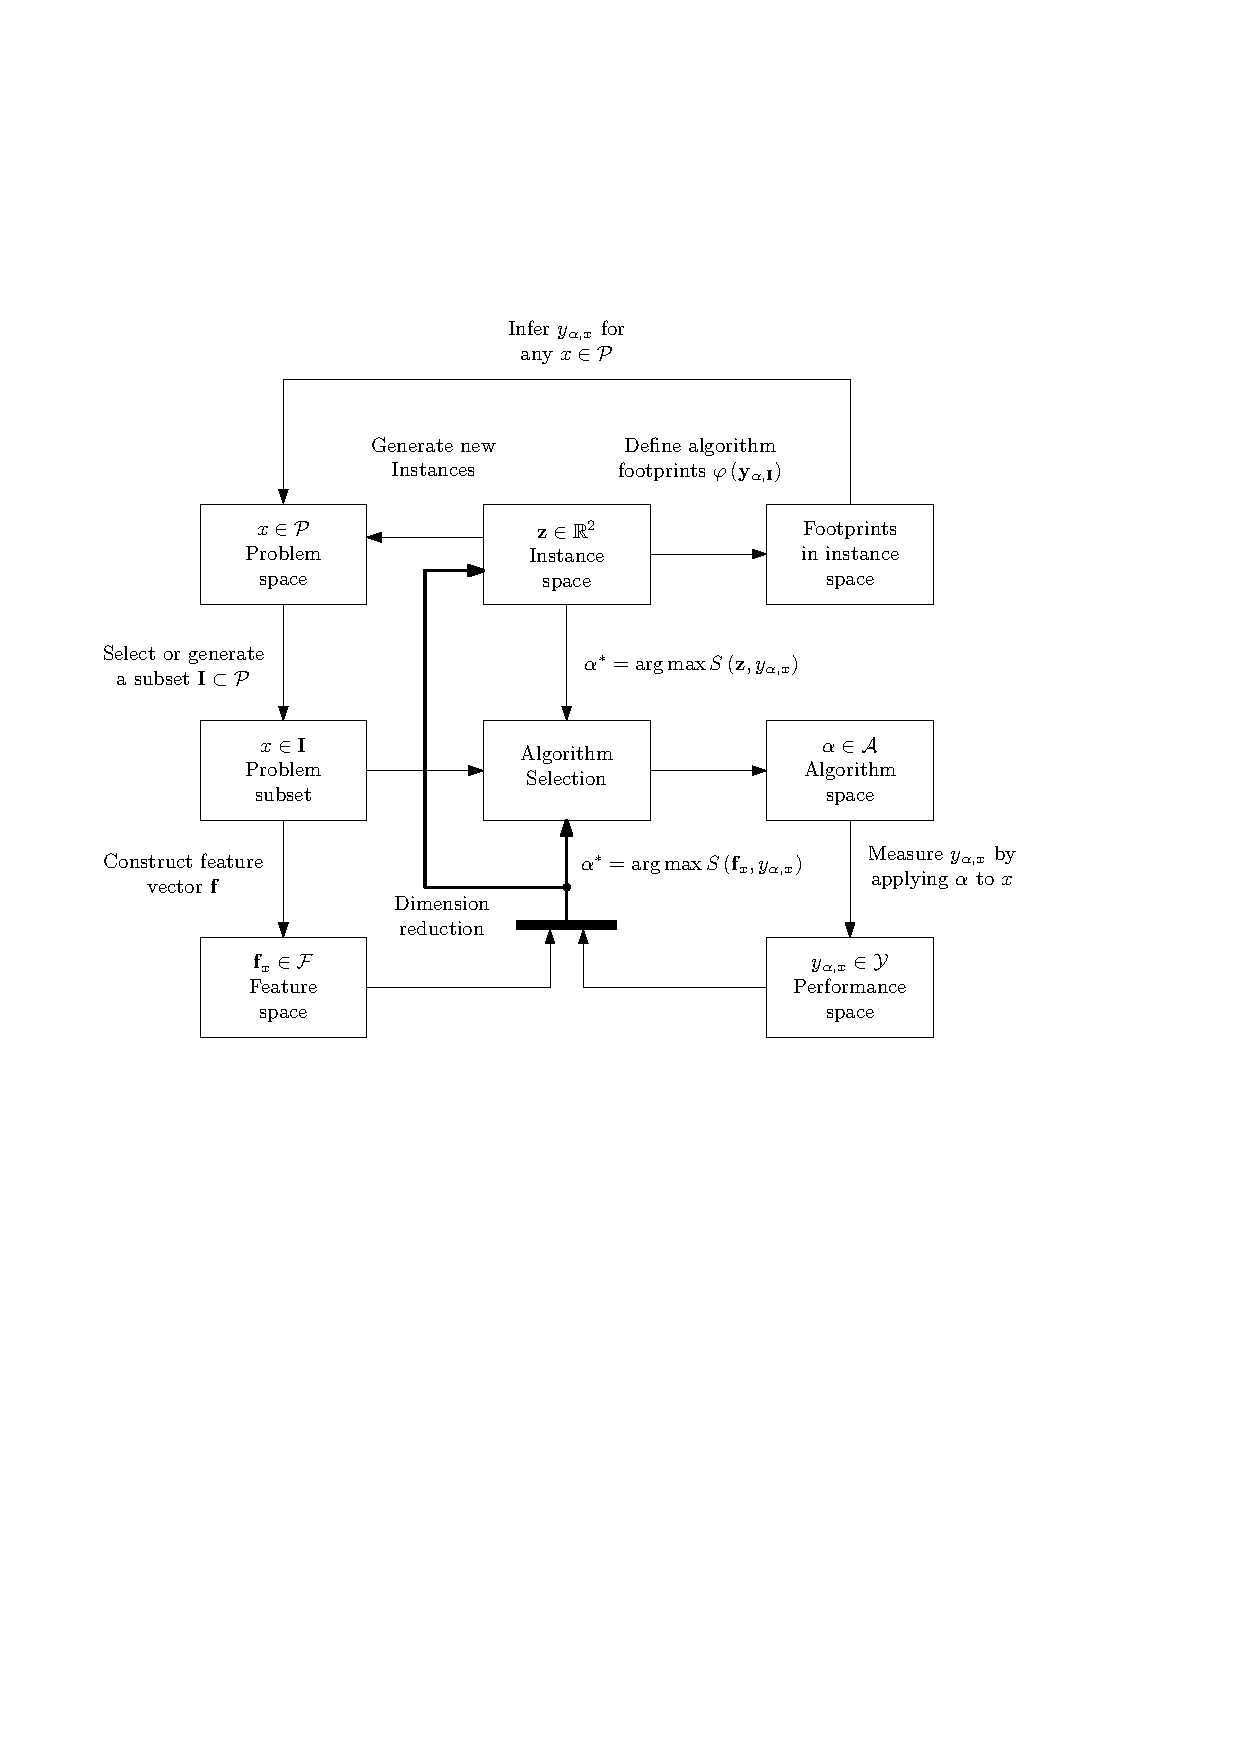
\includegraphics[width=0.90\textwidth, clip]{AlgorithmSelection3.pdf}
	\caption{Summary of the {ISA} framework~\protect\cite{SmithMiles2022}}
	\label{fig:AlgorithmSelection}
\end{figure}
% -----------------------------------------------------------------------

The features describe the similarities and differences among instances in $\Ibf$ and correlate with the performance of one or more algorithms. The features are calculated for a given instance $x$, and comprise the elements of the feature vector, $\f_{x}$, which represents an instance in the \textit{feature space}, $\Fcl$. The performance measure for an algorithm $\alpha$ describes the resources employed when solving an instance $x\in\Ibf$, where $\alpha$ is an element of the \textit{algorithm space}, $\Acl$, representing the set of algorithms available to solve all instances in $\Ibf$. The vector of performance measures, $y_{\alpha,x}$, describes the \textit{performance space}, $\Ycl$.

The meta-data can be used to learn a selection mapping, $S\left(\cdot\right)$, to identify the algorithm $\alpha^{*}$ most likely to be best for a given instance $x$, i.e., $\alpha^{*}=\arg\max\hspace{1mm}S\left(\f_{x},y_{\alpha,x}\right)$. Alternatively, the metadata can be used to map each instance from its $m$-dimensional feature vector to a point $\z$ in a $2D$ \textit{instance space}, allowing for visual inspection. Comparisons between algorithms are possible by estimating their \textit{footprints}, $\varphi\left(\y_{\alpha,\Ibf}\right)$, which are the regions in the instance space where we expect acceptable performance of the algorithm, where a threshold, $\epsilon$, defines the acceptability criteria. Footprints are characterised by their \textit{area}, which provides a measure of algorithm robustness; \textit{density}, which indicates the statistical strength of evidence; and \textit{purity}, which indicates whether there is conflicting evidence or not~\cite{SmithMiles2022}.

In the following sections, we present the experimental setup followed to build an instance space of neural network training tasks as black-box optimisation problems. The setup closely follows the one described in~\cite{Malan2025}, while introducing new dimensions and performance data. Both feature and algorithm performance data were collected using Python v3.10.4 on a high-performance computing environment, while post-processing was carried out in MATLAB R2025a. Code is available in GitHub\footnote{Available at \url{https://anonymous.4open.science/r/CORNN_TELO-CF88/}}, while raw and processed data are available in a Figshare collection\footnote{Due to limitations on how Figshare works, and to maintain anonymity, the data has been split into four items and made available through these URLs:
(a) \url{https://figshare.com/s/a46451b380cc31dac1f9} (b) \url{https://figshare.com/s/8517d08d0004a8efcfdf} (c) \url{https://figshare.com/s/a75bfb9deb27bbe59568}, and (d) \url{https://figshare.com/s/d81663e170efb83dae0f}. These will be consolidated in a single collection with a DOI once the paper is accepted. }.

% ===================================================================
\subsection{Problem instance subset}
% ===================================================================
Our instance subset comprises the CORNN suite~\cite{Malan2022} and the large-scale BBOB noiseless benchmark set from the Comparing Continuous Optimisers (COCO) platform~\cite{hansen2021coco}. For the CORNN suite, we consider the complete set of one-, three-, and five-layer networks, with dimensions 41, 261, and 482, respectively. As a result, we have a total of 648 CORNN instances (54 regression functions, each fitted using Tanh and ReLU activation functions, with one instance based on the training set and one based on the testing set, and three different dimensionalities), 216 per dimension. We used the \texttt{CORNN} package v0.9 and \texttt{PyTorch} v1.12.1.

For the large-scale BBOB set, we used the Python package v2.6.100, built from source, modifying the \texttt{`suite_largescale.c'} file to change the default dimensions from $\left\{20, 40, 80, 160, 320, 640\right\}$ to $\left\{41, 261, 482\right\}$, thereby matching the dimension of the CORNN suite instances. The COCO software uses 24 functions as instance generators, each identified by an integer in the set $\left\{1,\ldots,24\right\}$. A translation, rotation, oscillation, or a break in symmetry transforms each instance. For each basis function, we analysed 15 instances per dimension, yielding 1,080 BBOB instances (360 per dimension).

% ===================================================================
\subsection{Feature space}
% ===================================================================
We employed the \texttt{pflacco}~\cite{Prager2024} Python package v1.2.2 to calculate the ELA features, and followed the current best practice for extracting and pre-processing sample data for landscape analysis~\cite{Renau2020,Prager2023} from the two benchmark suites. We generated a single large input sample of $5\times100\times D$ observations, $\mathbf{X}$, using a Sobol set with scrambling via the MATLAB implementation of the Owen-inspired algorithm~\cite{Hong2003Algorithm823}. An advantage of using a Sobol set is typically higher convergence rates than purely random methods, due to its lower discrepancy. We then split this set into five sets of $100\times D$ observations. These sets, bounded between $\left[0,1\right]$, were scaled into $\left[-1,1\right]$ and stored as CSV files for the following stages of processing, and then scaled into $\left[-5,5\right]$ to be evaluated in the BBOB suite. Equal bounds were used for the CORNN suite, and we collected both the training and test responses. Finally, we standardised the responses for each instance using the mean and standard deviation. By sharing the input sample across instances, we remove the influence of sampling on the analysis and ensure that any observed differences are not due to sample size or sampling method. Moreover, sharing $\mathbf{X}$ reduces the overall computational cost, as no new observations were taken from the space.

From the ELA features available in the \texttt{pflacco} package, we did not use feature sets that require additional observations, such as local search and convexity. We also excluded the basic feature set, as these contained redundant information, and any feature that counted runtime or the number of additional function evaluations, since these are spurious. Likewise, features with large memory requirements, such as those that require cell-mapping, local linear models, and meta-models, were excluded for high-dimensional instances. 

Values were computed for the remaining ELA features for each subset of $100\times D$ observations, and these were then averaged to obtain a stable estimate. In~\cite{Malan2025}, five features ({\tt pca\_expl\_var\_cov\_x}, {\tt pca\_expl\_var\_cor\_x}, {\tt pca\_expl\_var\_PC1\_cov\_x}, and {\tt pca\_expl\_var\_PC1\_cor\_x}) had constant values across the instances; hence, they were removed from the set of features. However, in this study, we observed that the values were constant within dimensions but different across dimensions, so they were retained. This yielded a final set of 52 ELA features for the study.

% ===================================================================
\subsection{Algorithm and performance spaces}\label{sec:alg_perf}
% ===================================================================
Performance data was collected using the same four black-box algorithms used in the original CORNN suite paper~\cite{Malan2022}, i.e., CMA-ES, PSO, Two-Points DE, and Random Search, using the \texttt{nevergrad}~\cite{nevergrad2018} Python package v1.0.8. All algorithms were run 30 times per instance, with each run using 5~000 function evaluations. Performance was measured using the fixed-target approach~\cite{hansen2021coco}, where a run is successful if the algorithm reaches the target within the budget, and unsuccessful otherwise. Targets were set as a distance, in powers of 10, to the known optima and set between $\left[-1,1\right]$ at steps of 0.1, resulting in 21 targets, i.e., $\left\{10^{-1}, 10^{-0.9},\ldots,10^{-0.1},10^{0},10^{0.1},\ldots,10^{0.9},10^1\right\}$. Targets higher than 10.0 were deemed, on average, trivial, while targets lower than 0.10 were often unsolvable.

As a performance metric, we use the logarithm base-10 of the Expected Running Time (ERT) defined as the sum of the number of function evaluations ($F_{\text{evals}}$) required to reach a target value for successful runs, or the budget value for unsuccessful runs, divided by the number of successful runs. To summarise the results per instance, we compute the area under the curve (AUC) of the Empirical Cumulative Probability Distribution (ECDF) across all targets using the trapezoidal rule. We define our acceptability threshold as $\epsilon=0$, meaning that an algorithm is acceptable if it finds at least one target.

% ===================================================================
\subsection{Dimensionality reduction}\label{ssec:dimension_reduction}
% ===================================================================
To produce an instance space, rather than using the PILOT algorithm~\cite{SmithMiles2022} for dimensionality reduction, we combine PCA and t-SNE. We standardised the final feature set using the mean-standard deviation method and applied PCA to reduce the dimension from 52 to 14, retaining 99.50\% of the variance. Then, using t-SNE with Euclidean distance, perplexity of 30, and exaggeration of 4, we obtained the final 2$D$ embedding. We apply PCA before t-SNE to reduce computational cost and to address the assumption of local linearity, which may not hold in higher dimensions. While this approach does not incorporate performance information into the construction of the projection, as PILOT does, it can reveal local interactions among features that would otherwise be unobservable. We will examine the relationships between features and performance using correlation analysis.

To interpret the strength of influence of each feature on each axis of the visualisation and to understand which features better represent these instances, we computed Pearson correlations between the projected data and each raw ELA feature. To avoid focusing on a few highly intercorrelated features, we used the absolute value of the Pearson correlation as the similarity metric to identify feature groups. Then, we used t-SNE to generate a 2$D$ embedding of this similarity metric on which we applied K-Means clustering. Using the gap statistic by~\citet{tibshirani01gap}, we identified the best number of clusters $K$ by satisfying $\text{Gap}\left(K\right)\geq\text{Gap}\left(K+1\right)-\text{SE}\left(K+1\right)$, where $\text{SE}$ is the standard error of the clustering solution. These resulted in five clusters, of which four had features with at least a weak correlation (absolute value > 0.1) with either axis of the visualisation. We selected the highest-correlated features from these four clusters for the final analysis.

% ===================================================================
\subsection{Footprint analysis}
% ===================================================================
The final step in our instance space analysis is to calculate the footprints for both acceptable and best performance. In this paper, we use TRACE\textsuperscript{3}~\cite{Simpson2025}, which employs K-Nearest Neighbours (KNN) classification rather than DBSCAN to group instances into clusters. KNN closely aligns with the underlying intuition behind portfolio footprints, i.e., regions with similar feature values are expected to exhibit similar performance. TRACE\textsuperscript{3} follows these steps: 
\begin{inparaenum}[(a)]
    \item estimating the area and density of the convex hull containing all instances in $\Ibf$, which are used to scale individual footprints as a percentage of the complete instance space;
    \item constructing a KNN classifier for each algorithm;
    \item building $\alpha$-shape footprints from the KNN classifier predictions; and
    \item trimming outlier and sparse regions of the footprints.
\end{inparaenum}

We used the default parameters for TRACE\textsuperscript{3}~\cite{Simpson2025}, i.e., the number of nearest neighbours, $k$, is 50. At the same time, the radius for the $\alpha$-shapes is set to the minimum such that all valid instances, i.e., those whose input labels and KNN-predicted labels match, are included in the shape. We employ the TRACE\textsuperscript{3} implementation available at GitHub\footnote{\url{https://github.com/CSimpson4224/InstanceSpace3D}}, but provide a copy in our repository.

% ===================================================================
\section{Results}\label{sec:results}
% ===================================================================
We present three levels of results:
\begin{inparaenum}[(a)]
    \item First, we present the 2$D$ instance space visualisation from the perspective of the combined BBOB and CORNN suite instances;
    \item next, we provide an analysis of the individual ELA features; and
    \item finally, we present an analysis of the performance of four black-box algorithms on the instances.
\end{inparaenum}
% ===================================================================
\subsection{Instance space structure}
% ===================================================================

% -----------------------------------------------------------------------
%
% -----------------------------------------------------------------------
\begin{figure*}[!t]
    \centering
    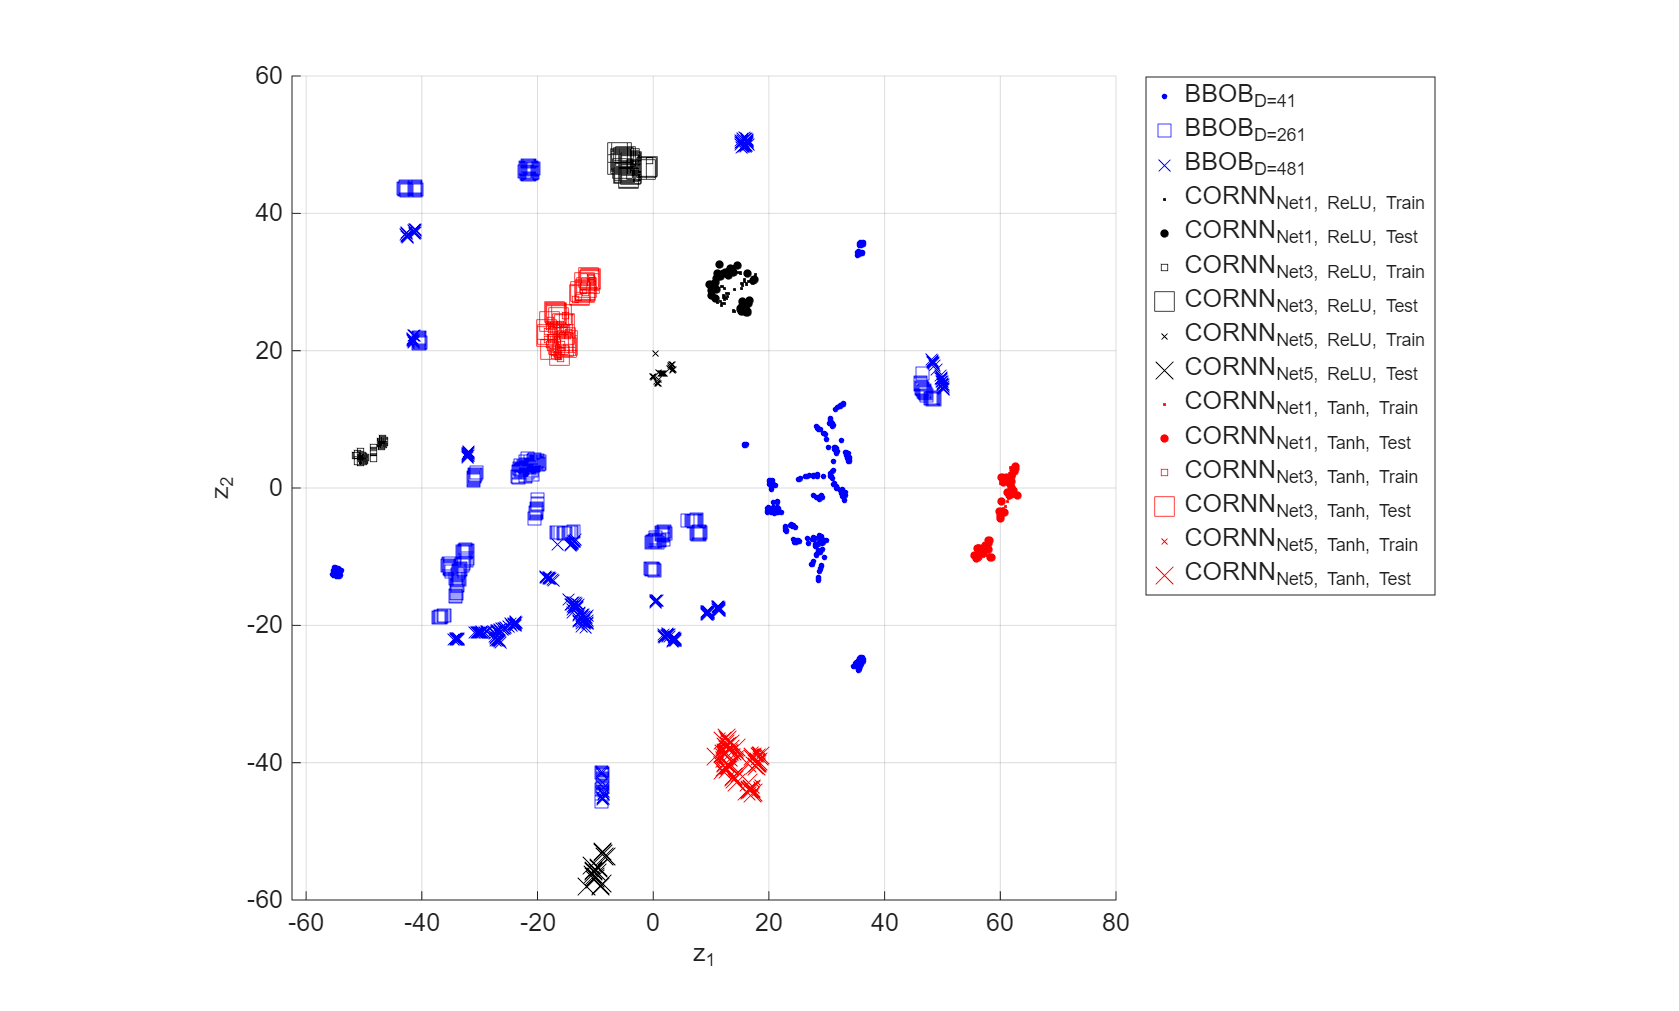
\includegraphics[trim=3.5cm 0.5cm 3.5cm 1.0cm, clip=true, width = 0.90\textwidth]{bbob_cornn_by_dimension.png}
    \caption{A 2$D$ instance space of the BBOB and CORNN suites, separated by dimensionality (41, 261, and 481), activation function (ReLU and Tanh), and dataset (Train and Test). The figure demonstrates that the CORNN instances are distinctive from the BBOB ones. Both suites show differences in dimensionality. There are noticeable structural differences between train and test CORNN instances with the ReLU activation function.}
	\label{fig:bbob_cornn_by_dimension}
\end{figure*}
% -----------------------------------------------------------------------
%
% -----------------------------------------------------------------------
\begin{figure*}[!p]
    \centering
    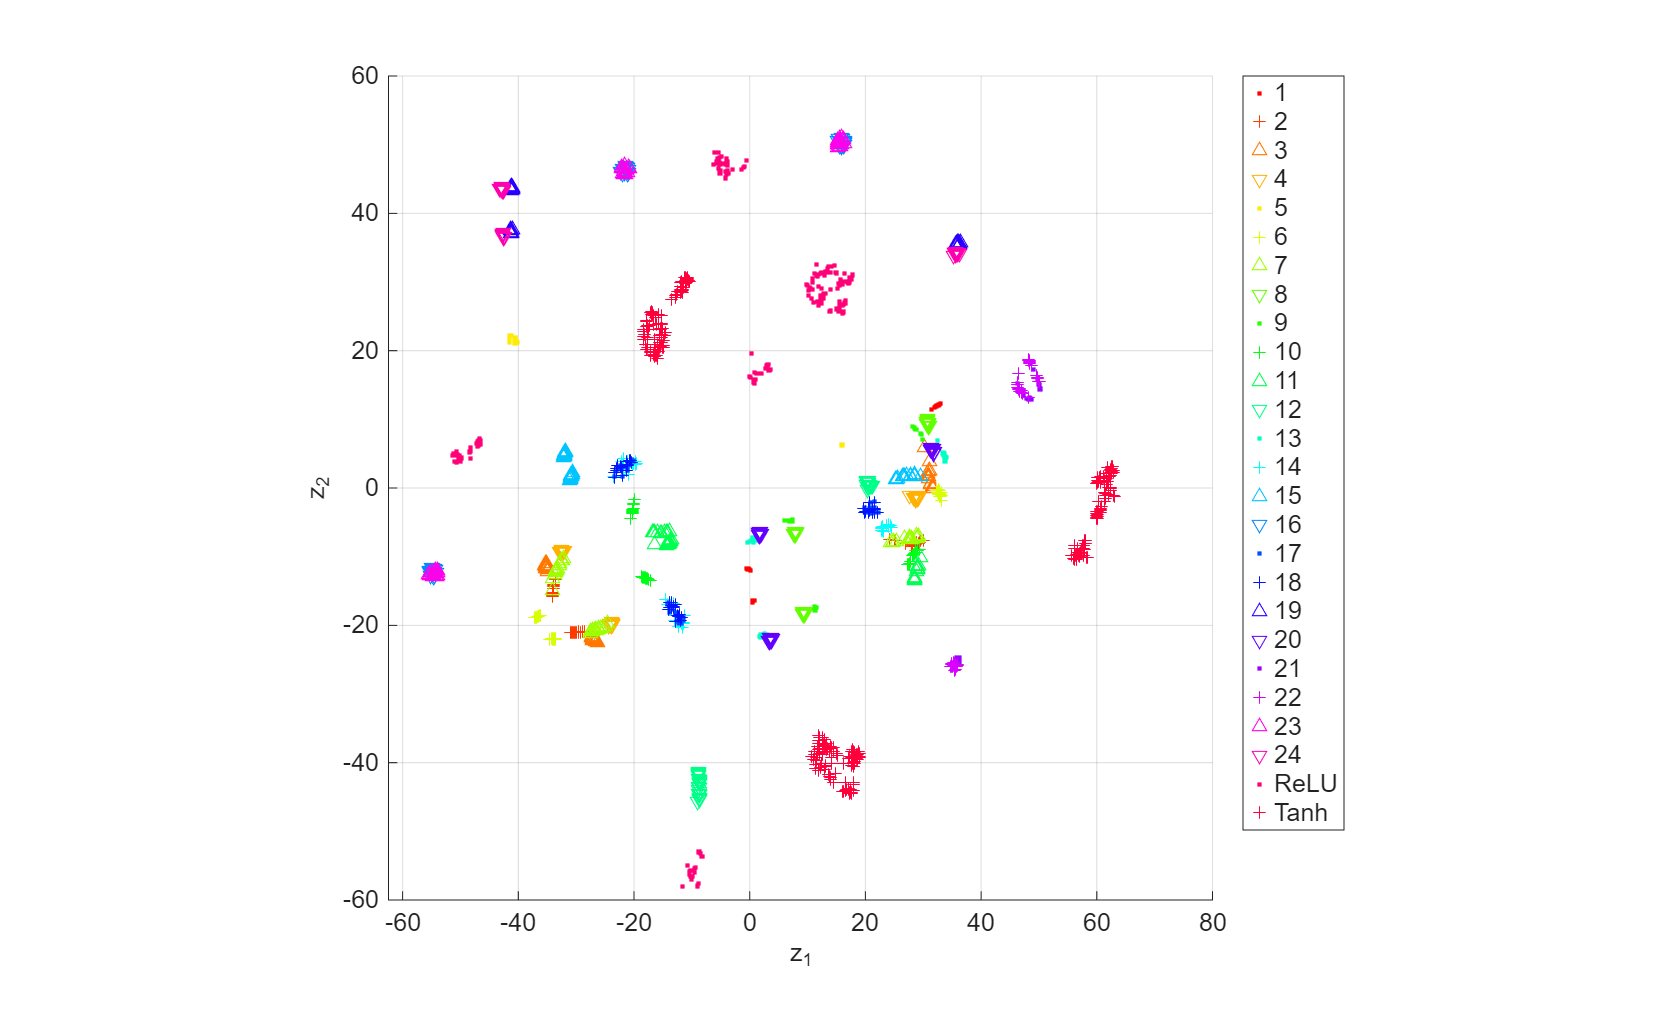
\includegraphics[trim=3.5cm 0.5cm 3.5cm 1.0cm, clip=true, width = 0.90\textwidth]{bbob_cornn_by_function.png}
    \caption{A 2$D$ Instance Space of the BBOB and CORNN suites, separated by their generating function. The figure demonstrates the existence of some peripheral BBOB instances generated by functions $\left\{12,16,19,21,23,24\right\}$.}
	\label{fig:bbob_cornn_by_function}
\end{figure*}
% -----------------------------------------------------------------------
%
% -----------------------------------------------------------------------
\begin{figure*}[!p]
    \centering
    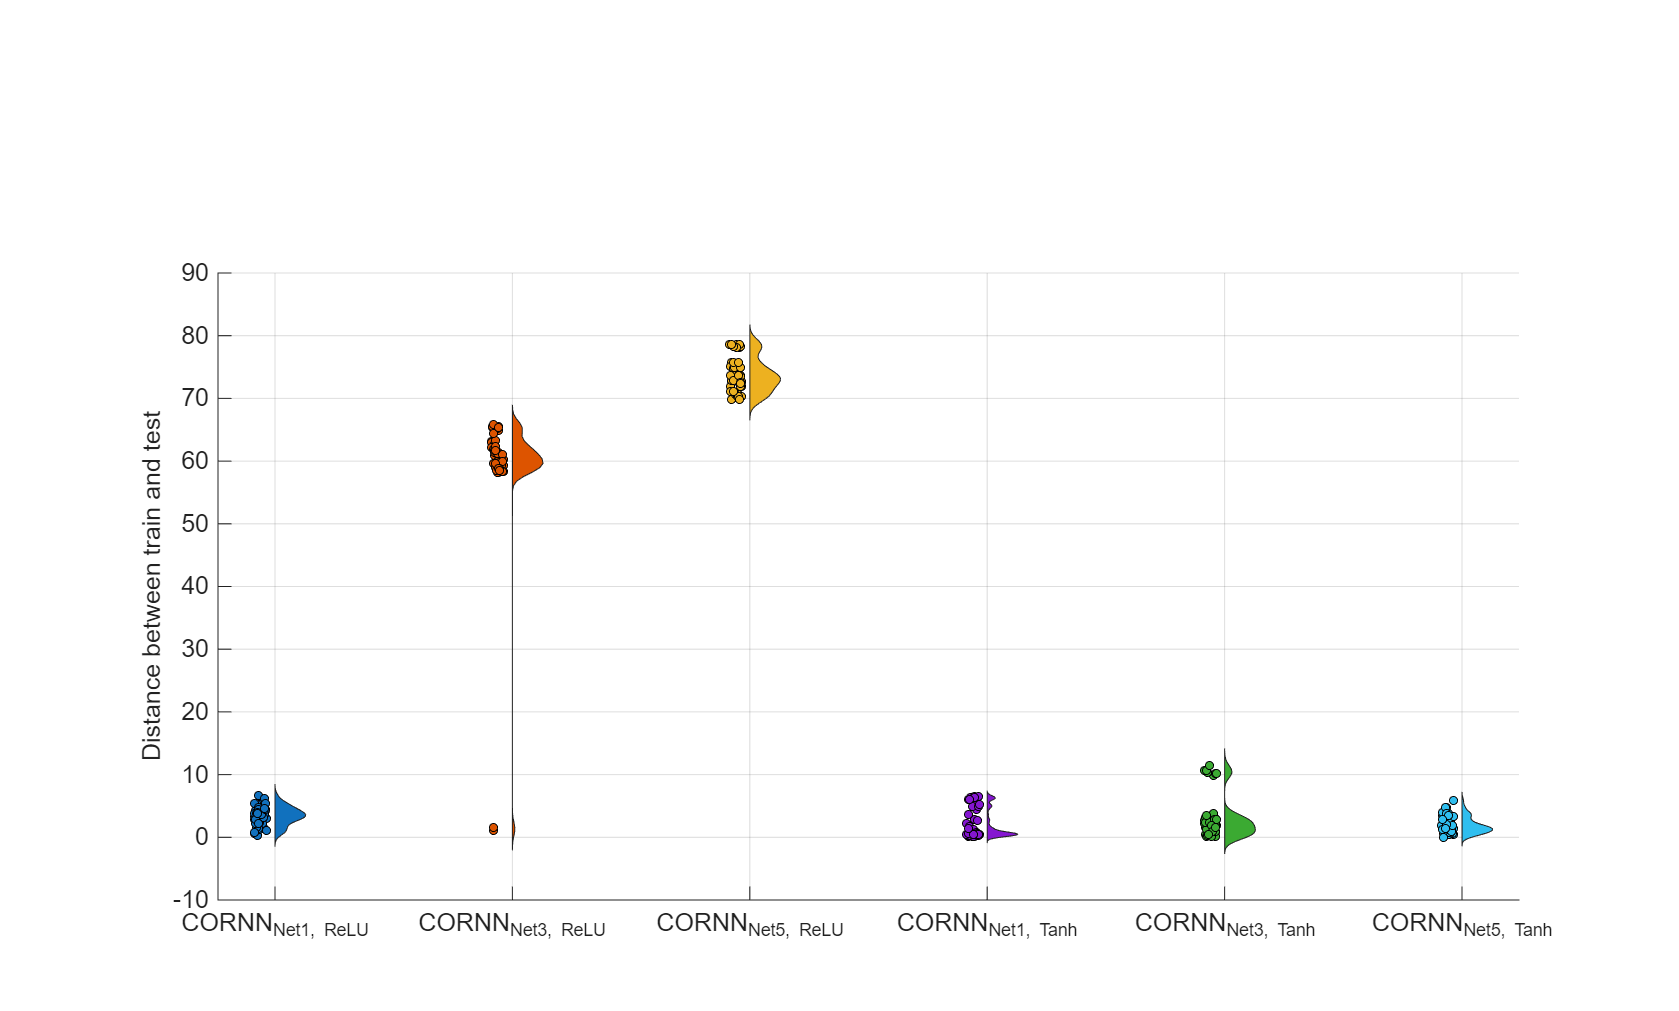
\includegraphics[trim=2.0cm 1.0cm 1.5cm 4.0cm, clip=true, width = 0.90\textwidth]{train_test_distance_by_groups.png}
    \caption{Distribution of the distance within the 2$D$ Instance Space between the training and test instances for the same regression problem. The instances have been separated by layer and activation function. The figure illustrates the structural differences among the multi-layered, train, and test CORNN instances with the ReLU activation function.}
	\label{fig:train_test_distance_by_groups}
\end{figure*}
% -----------------------------------------------------------------------

Figure~\ref{fig:bbob_cornn_by_dimension} illustrates the resulting instance space, where the colour represents the benchmark suite, i.e., blue for BBOB, black and red for CORNN; the mark shape indicates the dimensionality, i.e., dots for $D=41$, squares for $D=261$ and crosses for $D=481$; and the size the data source for the regression problem, i.e., small for train, large for test. Meanwhile, Figure~\ref{fig:bbob_cornn_by_function} colour-codes the individual generating functions.

A few observations are noteworthy. First, there is a clear separation between the BBOB and CORNN instances across all dimensions, with a set of `core' clusters roughly between $\left[-40,40\right]$ on the horizontal axis and $[-20,20]$ on the vertical axis formed by most BBOB instances, and several peripheral clusters comprising both CORNN and some BBOB instances belonging to functions $\left\{12,16,19,21,23,24\right\}$, mostly aligning with the observations from~\cite{Malan2025} (limited to 41$D$ instances), where the peripheral BBOB functions where $\left\{9, 16, 19, 21, 22, 23, 24\right\}$. Using the qualitative descriptors of these BBOB functions by~\citet{Mersmann2010}, these functions tend to have weak or no global structure and low-to-medium global-to-local contrast. The former indicates the absence of a main global funnel, while the latter suggests no difference between local and global optima. These observations generally align with our expectations for the structure of neural network training tasks, where we anticipate finding no global structure and multiple global optima due to symmetry. Moreover, these properties remain regardless of the increase in dimensionality.

Second, while CORNN instances with the Tanh activation function tend to cluster together, regardless of dimension, as observed in~\cite{Malan2025}, those with the ReLU activation function tend to separate between training and test instances, with the effect becoming more pronounced in higher dimensions. There is no significant difference being induced by the underlying regression problem. 
% Note that the ReLU activation function maps all negative inputs to zero, thereby introducing neutrality in the network's output and the associated error landscape. On the other hand, the Tanh function has a near-vertical gradient at zero, leading to significant differences in the outputs of neighbouring weight vectors at this point. This could lead to sharper changes in the neural network's error landscape. While this explains the differences between activation functions, it does not explain the difference between training and test instances for ReLU. 


% We also note that within each activation function class, the problem instances in the CORNN suite appear very similar. This could mean that the instances share similar landscapes, but it is more likely due to limitations in the ELA characterisation. ELA metrics do not explicitly measure specific landscape features, such as neutrality and steep gradients, which may better distinguish between CORNN instances. Further experimentation is required to confirm this.

To confirm the observation of a difference between training and testing instances for ReLU, we examine the distance between the train and test instances for the same regression problem. Figure~\ref{fig:train_test_distance_by_groups} illustrates the distribution of the Euclidean distance within the projection between train and test instances as violin plots. Generally, the training and test instances with Tanh are closer to each other, with median distances of 0.704 units for $D=41$, 1.858 for $D=261$, and 1.466 for $D=481$. In contrast, for ReLU, the median distance is 3.590 units for $D=41$, 60.302 for $D=261$, and 73.480 for $D=481$, all of which are higher than for the highest median for Tanh. % [ANDRES: ARE THERE DIFFERENCES BETWEEN REGRESSION PROBLEMS?]

We hypothesise that the difference between the feature profiles of training and testing error landscapes for larger ReLU networks hints at problem instances that will be harder for algorithms to perform well on. In other words, for the 3-layer and 5-layer CORNN instances, the ReLU activation function leads to a disconnect between the training and testing landscapes (not observed with Tanh), which could negatively affect the network's ability to generalise to unseen data. It would be interesting to investigate whether this is a general phenomenon and to understand the underlying mechanism that causes this disconnect. % [ANDRES: please check that you agree with previous statements from "We hypothesise ...". I cannot explain why, so I have said something about the implication. Unless the performance is informing the instance space (like with PILOT)? From your description it seems not?]


% ===================================================================
\subsection{Individual feature analysis}
% ===================================================================
Table~\ref{tab:feature_clusters} presents the groups of highly intercorrelated features obtained through K-Means clustering on a 2$D$ embedding with Pearson correlation as similarity metric. In boldface are the features selected for further analysis using the method described in Section~\ref{ssec:dimension_reduction}. For interest, instances marked with $\left(*\right)$ are those selected in~\cite{Malan2025}, while those marked with $\left(\times\right)$ were the features identified by~\citet{Long2022} in their crashworthiness optimisation study. Of the features selected in~\cite{Malan2025}, {\tt ela\_level\_mmce\_qda\_25} belongs to Cluster 3 from which two other features were selected; {\tt ic\_eps\_max} belongs to Cluster 2 from which two other features were also selected; {\tt limo\_avg\_length\_reg} was not calculated due to computational constraints; and {\tt nbc\_nb\_fitness\_cor} belongs to Cluster 4, from which this and another feature were selected. In contrast, the features selected in~\cite{Long2022}, {\tt pca\_expl\_var\_PC1\_cor\_x} and {\tt pca\_expl\_var\_PC1\_cor\_init} belong to Cluster 2, and {\tt ela\_meta\_lin\_w\_interact\_adj\_r2} was also not calculated due to computational constraints.

% -----------------------------------------------------------------------
%
% -----------------------------------------------------------------------
\begin{table}[!t]
    \caption{Clusters of highly intercorrelated features. Features in boldface were selected based on their correlation with the instance space axes; those marked with \textsuperscript{$\left(*\right)$} were identified in~\protect\cite{Malan2025}, while those marked with \textsuperscript{($\times$)} were identified as significant in the~\protect\citet{Long2022} study.}
    \label{tab:feature_clusters}
    \footnotesize
    \begin{tabular}{l>{\raggedright\arraybackslash}p{11.5cm}}
        \toprule
        Cluster 1 & {\tt disp\_diff\_mean\_02, disp\_diff\_mean\_05, disp\_diff\_mean\_10, \textbf{disp\_diff\_mean\_25}, disp\_diff\_median\_02, disp\_diff\_median\_05, disp\_diff\_median\_10, disp\_diff\_median\_25,  nbc\_nn\_nb\_sd\_ratio, \textbf{nbc\_nn\_nb\_cor} } \\
        \midrule
        
        Cluster 2 & {\tt ic\_eps\_s, {ic\_eps\_max}\textsuperscript{(*)}, ic\_eps\_ratio, nbc\_nn\_nb\_mean\_ratio, nbc\_dist\_ratio\_coeff\_var, \textbf{pca\_expl\_var\_cov\_x}, pca\_expl\_var\_cor\_x, pca\_expl\_var\_cov\_init, pca\_expl\_var\_cor\_init, pca\_expl\_var\_PC1\_cov\_x, {pca\_expl\_var\_PC1\_cor\_x}\textsuperscript{($\times$)}, pca\_expl\_var\_PC1\_cov\_init, {pca\_expl\_var\_PC1\_cor\_init}\textsuperscript{($\times$)}, \textbf{fitness\_distance\_distance\_mean}} \\
        \midrule
        
        Cluster 3 & {\tt ela\_level\_mmce\_lda\_10, \textbf{ela\_level\_mmce\_qda\_10}, ela\_level\_lda\_qda\_10, ela\_level\_mmce\_lda\_25, {ela\_level\_mmce\_qda\_25}\textsuperscript{(*)}, ela\_level\_lda\_qda\_25, {ela\_level\_mmce\_lda\_50}, ela\_level\_mmce\_qda\_50, \textbf{ela\_level\_lda\_qda\_50}, ic\_m0} \\
        \midrule
        
        Cluster 4 & {\tt ela\_distr\_skewness, \textbf{ela\_distr\_kurtosis}, ela\_distr\_number\_of\_peaks, ic\_h\_max, \textbf{nbc\_nb\_fitness\_cor}\textsuperscript{(*)}, fitness\_distance\_fd\_cov, fitness\_distance\_fitness\_mean, fitness\_distance\_fitness\_std} \\
        \midrule
        
        Cluster 5 & {\tt disp\_ratio\_mean\_02, disp\_ratio\_mean\_05, disp\_ratio\_mean\_10, \textbf{disp\_ratio\_mean\_25}, \textbf{disp\_ratio\_median\_02}, disp\_ratio\_median\_05, disp\_ratio\_median\_10, disp\_ratio\_median\_25, fitness\_distance\_fd\_correlation, fitness\_distance\_distance\_std} \\
        \bottomrule
    \end{tabular}
\end{table}
% -----------------------------------------------------------------------

Table~\ref{tab:correlation_with_axes} presents the correlation between the selected features, the axes of the instance space, and the algorithm performance. In boldface, we mark the features that we will analyse in detail, selecting one feature from each cluster with the highest overall correlation. Although {\tt pca\_expl\_var\_cov\_x} and {\tt fitness\_distance\_distance\_mean} were selected, we do not continue with them because they provided little variation within dimensions, offering negligible additional information.

% -----------------------------------------------------------------------
%
% -----------------------------------------------------------------------
\begin{table}[!t]
	\centering
	\caption{Correlation between the ELA features selected in Table~\ref{tab:feature_clusters} and the axis of the instance space and algorithm performance. Features selected for further examination are shown in boldface.}
	\footnotesize
	\begin{tabular}{clrrrrrr}
        \toprule
        Cluster & Feature                                    & $z_{1}$        & $z_{2}$        & CMA            & PSO             & RandomSearch    & TwoPointsDE     \\
        \midrule
        \multirow{2}{*}{1} & {\tt disp\_diff\_mean\_25}                       & -0.193          & -0.146          & 0.451          & 0.445           & 0.467           & 0.540  \\
         & {\tt \textbf{nbc\_nn\_nb\_cor}}                  & -0.303 & -0.059          & -0.479         & \textbf{-0.529} & \textbf{-0.562} & \textbf{-0.562} \\ \midrule

        \multirow{2}{*}{2} & {\tt pca\_expl\_var\_cov\_x}                     & 0.591  & 0.127           & 0.023          & 0.144           & 0.150           & 0.045           \\
         & {\tt {fitness\_distance\_distance\_mean}} & {-0.498} & {-0.241} & 0.005          & -0.109          & -0.111          & -0.012 \\ \midrule

        \multirow{2}{*}{3} & {\tt \textbf{ela\_level\_mmce\_qda\_10}}         & -0.106          & \textbf{0.217}  & \textbf{0.581} & 0.486           & \textbf{0.532}  & \textbf{0.602}  \\
         & {\tt ela\_level\_lda\_qda\_50}                   & 0.470           & 0.137           & 0.238          & 0.265           & 0.287           & 0.244           \\ \midrule
        
        \multirow{2}{*}{4} & {\tt ela\_distr\_kurtosis}                       & -0.047          & -0.226          & 0.004          & -0.113          & -0.114          & -0.012 \\
         & {\tt \textbf{nbc\_nb\_fitness\_cor}}             & -0.285          & -0.179          & \textbf{0.527} & 0.113           & 0.170           & \textbf{0.520}  \\ \midrule

        \multirow{2}{*}{5} & {\tt disp\_ratio\_mean\_25}                      & -0.486          & -0.181          & 0.262          & 0.238           & 0.240  & 0.308           \\
         & {\tt \textbf{disp\_ratio\_median\_02}}           & \textbf{-0.502} & -0.157          & 0.279          & 0.224           & 0.237           & 0.318           \\
         \bottomrule        
	\end{tabular}
	\label{tab:correlation_with_axes}
\end{table}
% -----------------------------------------------------------------------

Figure~\ref{fig:violin_strong_features} illustrates the variation in values between the BBOB and CORNN instances of the four selected ELA features. The plots show that CORNN generally has low to medium values for {\tt nbc\_nn\_nb\_cor} compared to BBOB, and medium to high values for {\tt ela\_level\_mmce\_qda\_10}, {\tt nbc\_nb\_fitness\_cor} and {\tt disp\_ratio\_median\_02}. Moreover, these results show differences between ReLU and Tanh instances, with the former having generally higher values of {\tt nbc\_nn\_nb\_cor} and {\tt nbc\_nb\_fitness\_cor}, while lower values for {\tt disp\_ratio\_median\_02}. % However, {\tt fitness\_distance\_distance\_mean} shows a broad set of values for all functions, with some variation within dimensions. Therefore, to better observe these patterns, we will standardise the data across dimensions.

% -----------------------------------------------------------------------
%
% -----------------------------------------------------------------------
\begin{figure}[!t]
    \centering
    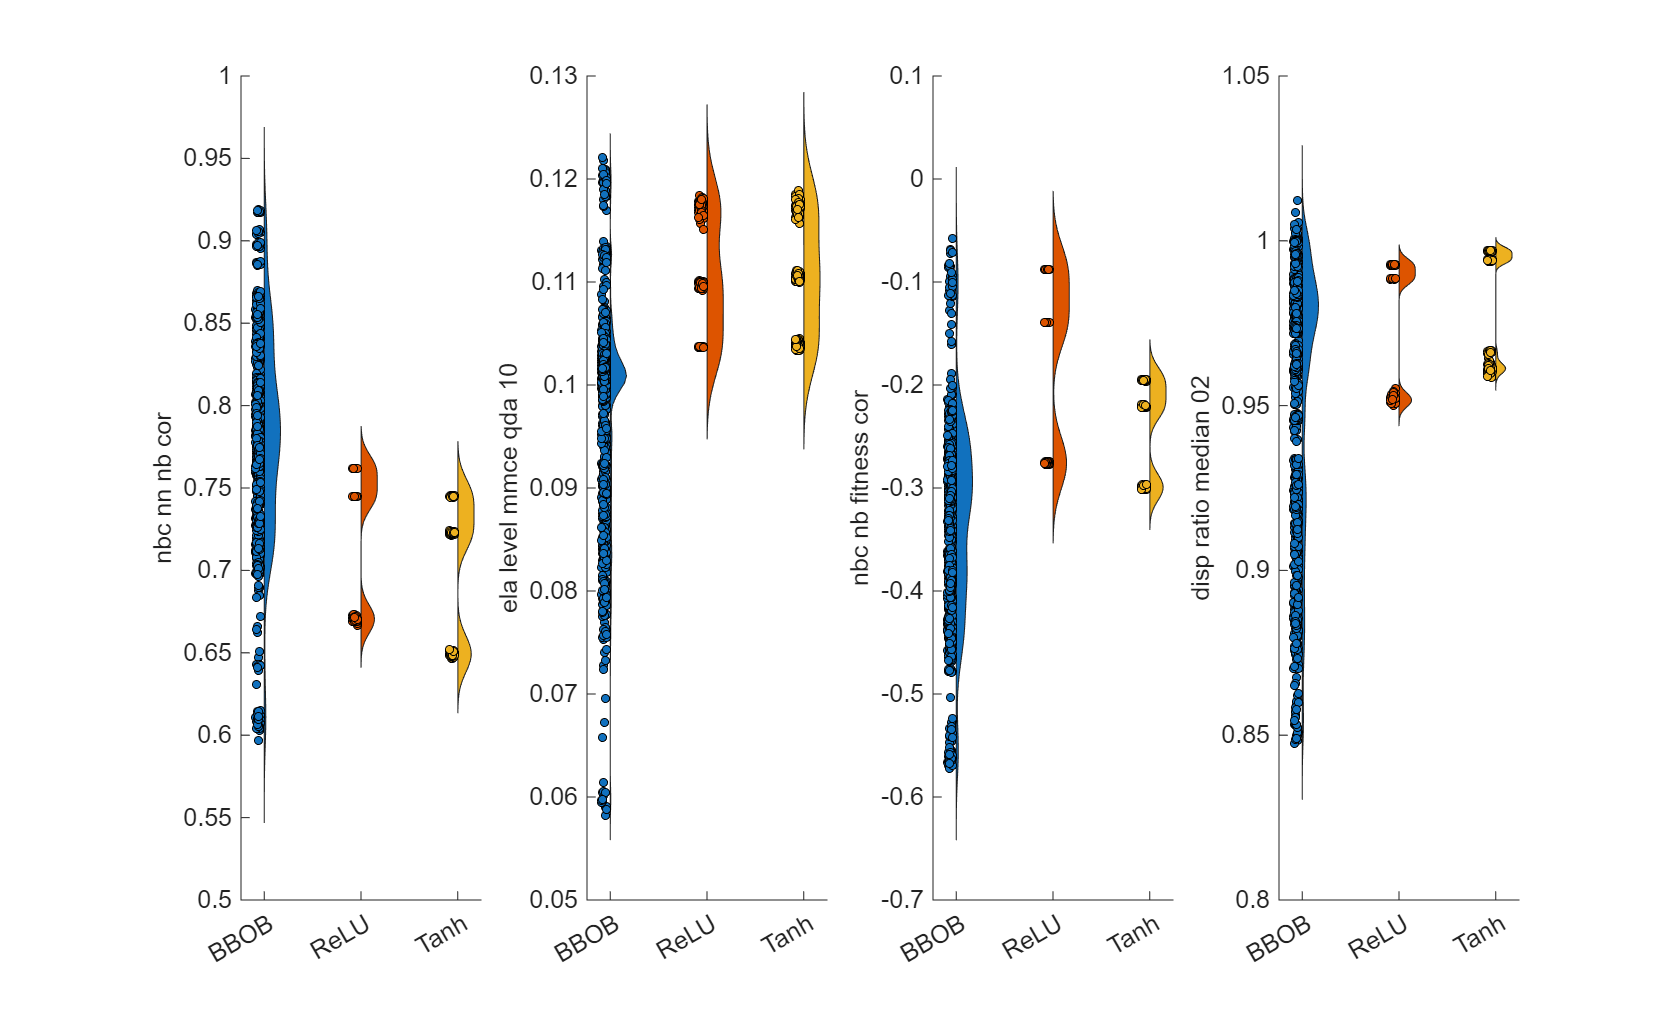
\includegraphics[trim=2.5cm 0.5cm 2.5cm 1.0cm, clip=true, width = 0.90\textwidth]{violin_strong_features.png}
    \caption{Violin plots of the ELA features with the highest correlation with the instance space axes. Analysis of variance indicates that the means across groups differ. The ranges for the CORNN instances are narrower.}
	\label{fig:violin_strong_features}
\end{figure}
% -----------------------------------------------------------------------

Let us examine the relationship between instances and features in more detail. Figure~\ref{fig:projection_by_features} illustrates the ELA feature values across the instance space, where we have differentiated CORNN instances from BBOB instances using grey boxes in the first plot. First, {\tt nbc\_nn\_nb\_cor} measures the correlation between the distance to the nearest neighbours and the distance to the nearest-better solutions, where the expectation is that in a funnel setting, the correlation should be high. In contrast, in a random peaks setting, it should be lower~\cite{Kerschke2015}. That is, the feature can be interpreted as measuring the degree of global structure in a landscape. Figure~\ref{fig:tsne_nbc_nn_nb_cor} shows that the BBOB functions cover the full range of values for this feature, with the lowest value corresponding to the BBOB function 23 -- Katsuura function with $D=41$, distributed in a cluster roughly at $\left[-55,-11\right]$, and described as ``Highly rugged and highly repetitive function, with more than $10^{D}$ global optima''~\cite{hansen:BBOB}. In contrast to BBOB, the CORNN suite instances all have low-to-medium values, aligning with our expectation that a lack of global structure and multiple optima characterise these search spaces. 

% -----------------------------------------------------------------------
%
% -----------------------------------------------------------------------
\begin{figure*}[!t]
    % \flushleft
    \subfloat[nbc\_nn\_nb\_cor]{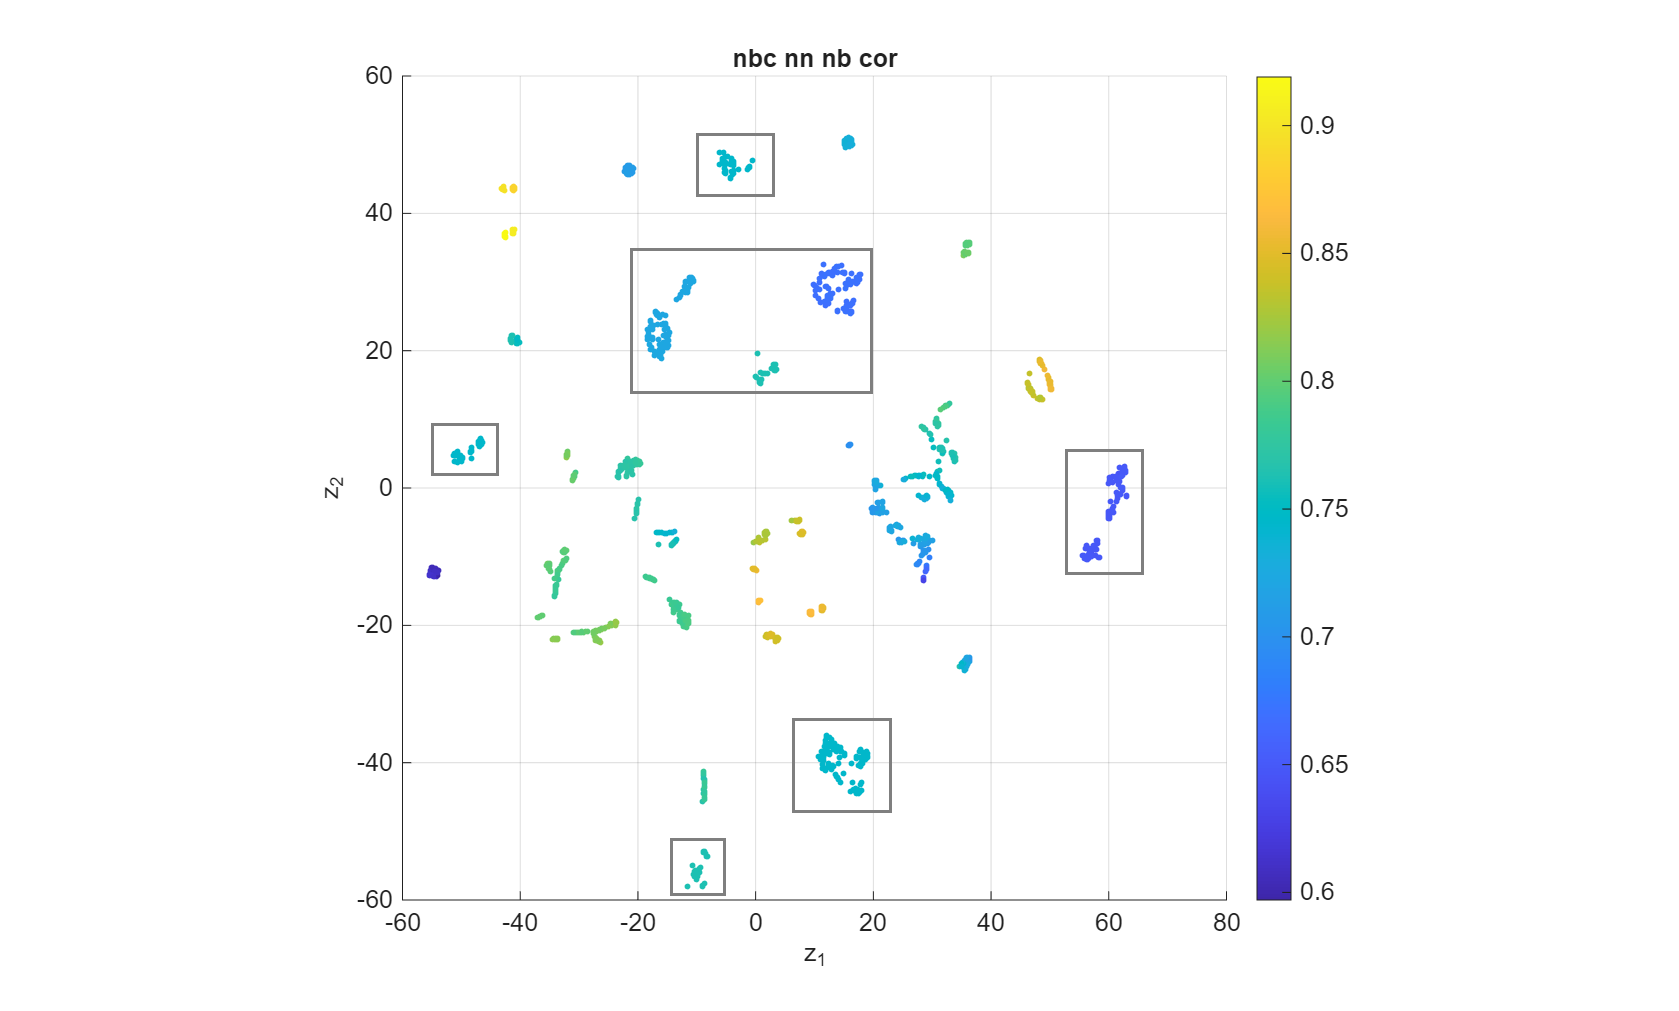
\includegraphics[trim=5.5cm 0.0cm 5.5cm 0.0cm, clip=true, width = 0.47\textwidth]{tsne_nbc_nn_nb_cor_annotate.png}\label{fig:tsne_nbc_nn_nb_cor}}
    % \subfloat[fitness\_distance\_distance\_mean]{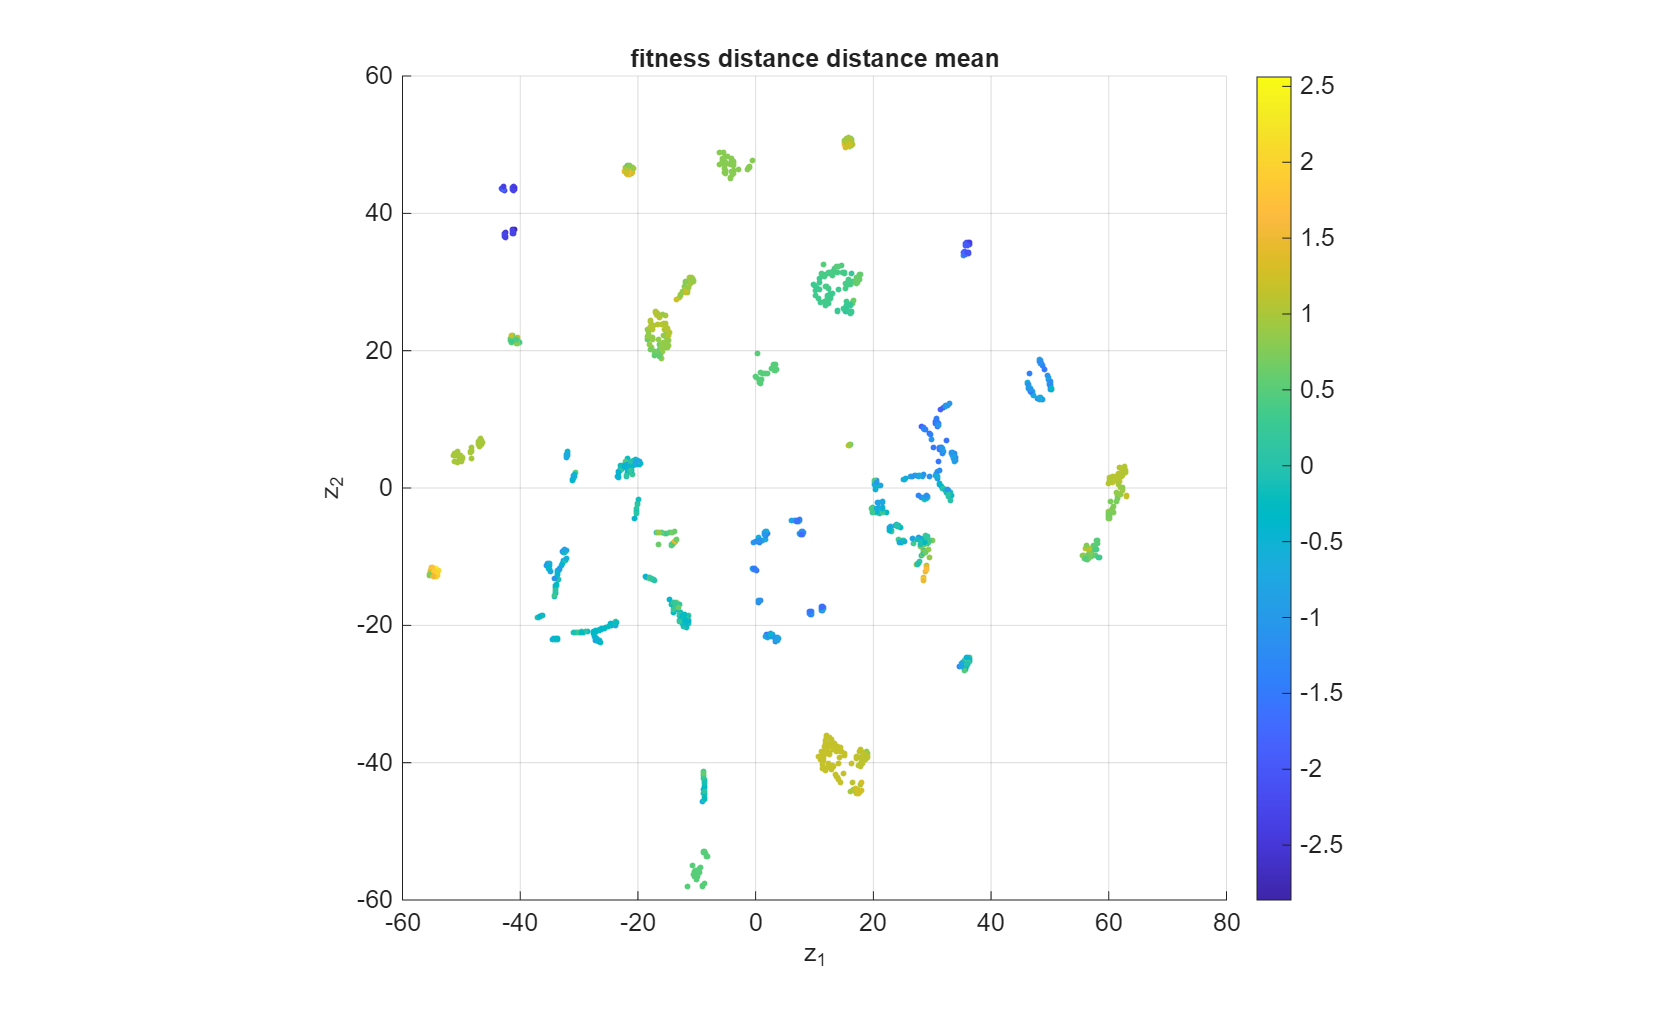
\includegraphics[trim=5.5cm 0.0cm 5.5cm 0.0cm, clip=true, width = 0.33\textwidth]{tsne_fitness_distance_distance_mean.png}\label{fig:tsne_fitness_distance_distance_mean}}
    \subfloat[ela\_level\_mmce\_qda\_10]{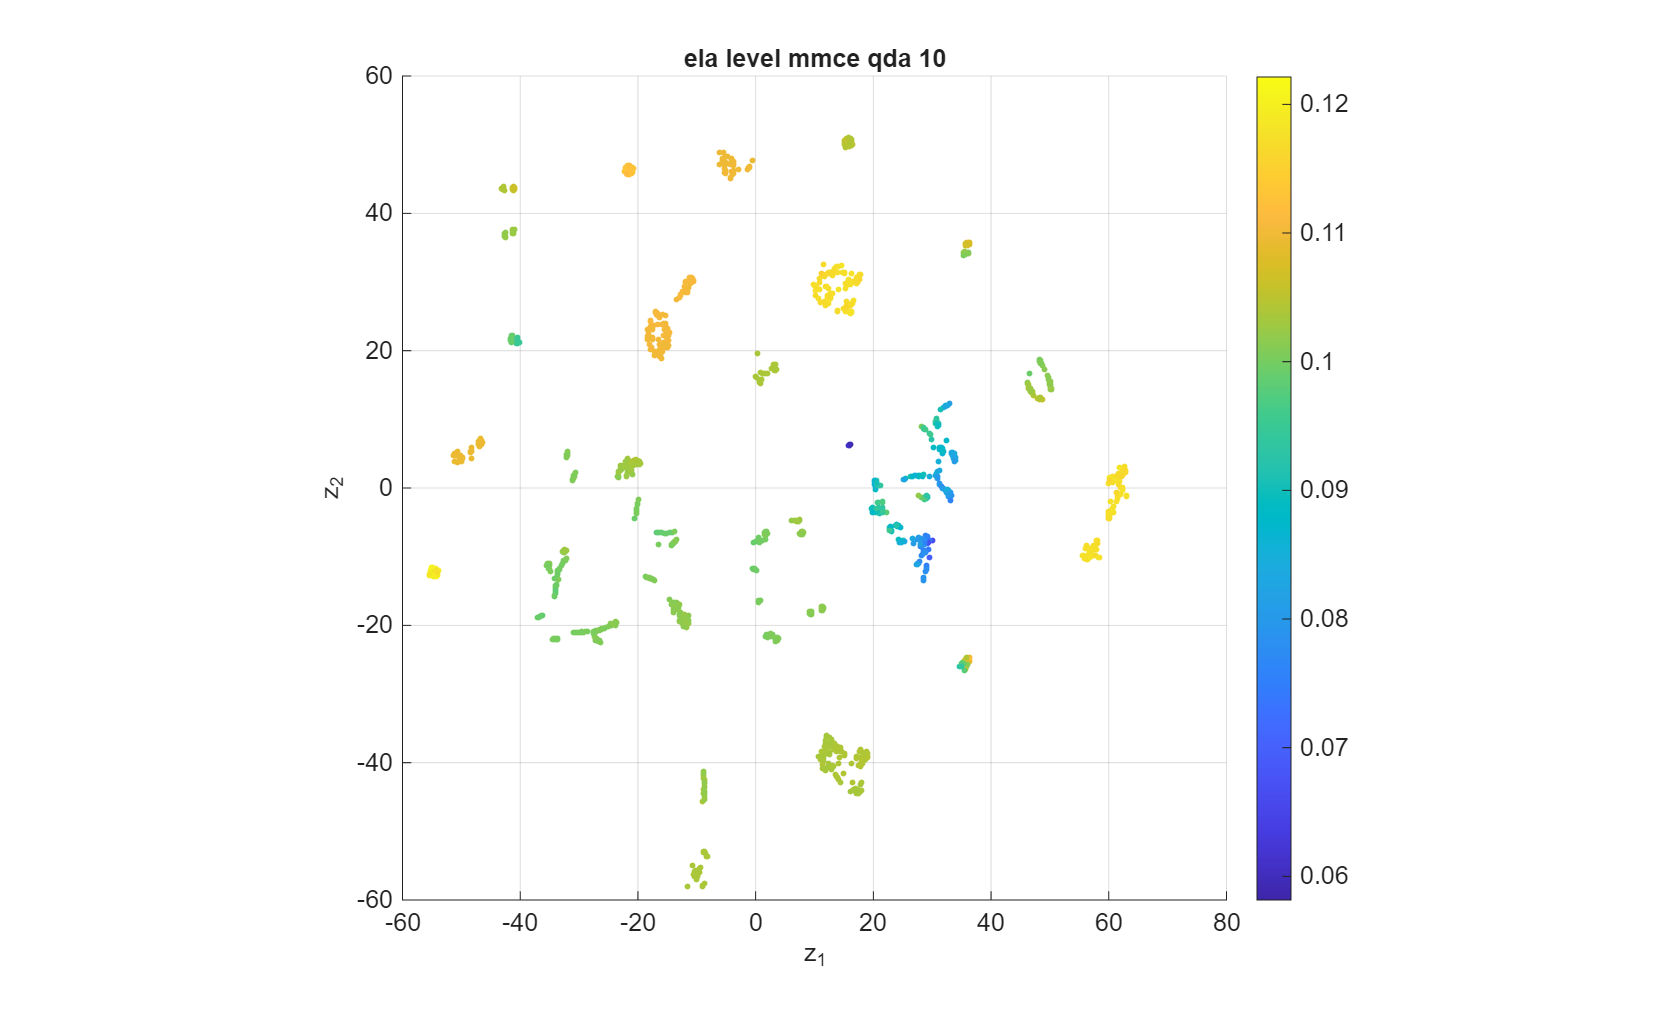
\includegraphics[trim=5.5cm 0.0cm 5.5cm 0.0cm, clip=true, width = 0.47\textwidth]{tsne_ela_level_mmce_qda_10.png}\label{fig:tsne_ela_level_mmce_qda_10}}\\
    \subfloat[nbc\_nb\_fitness\_cor]{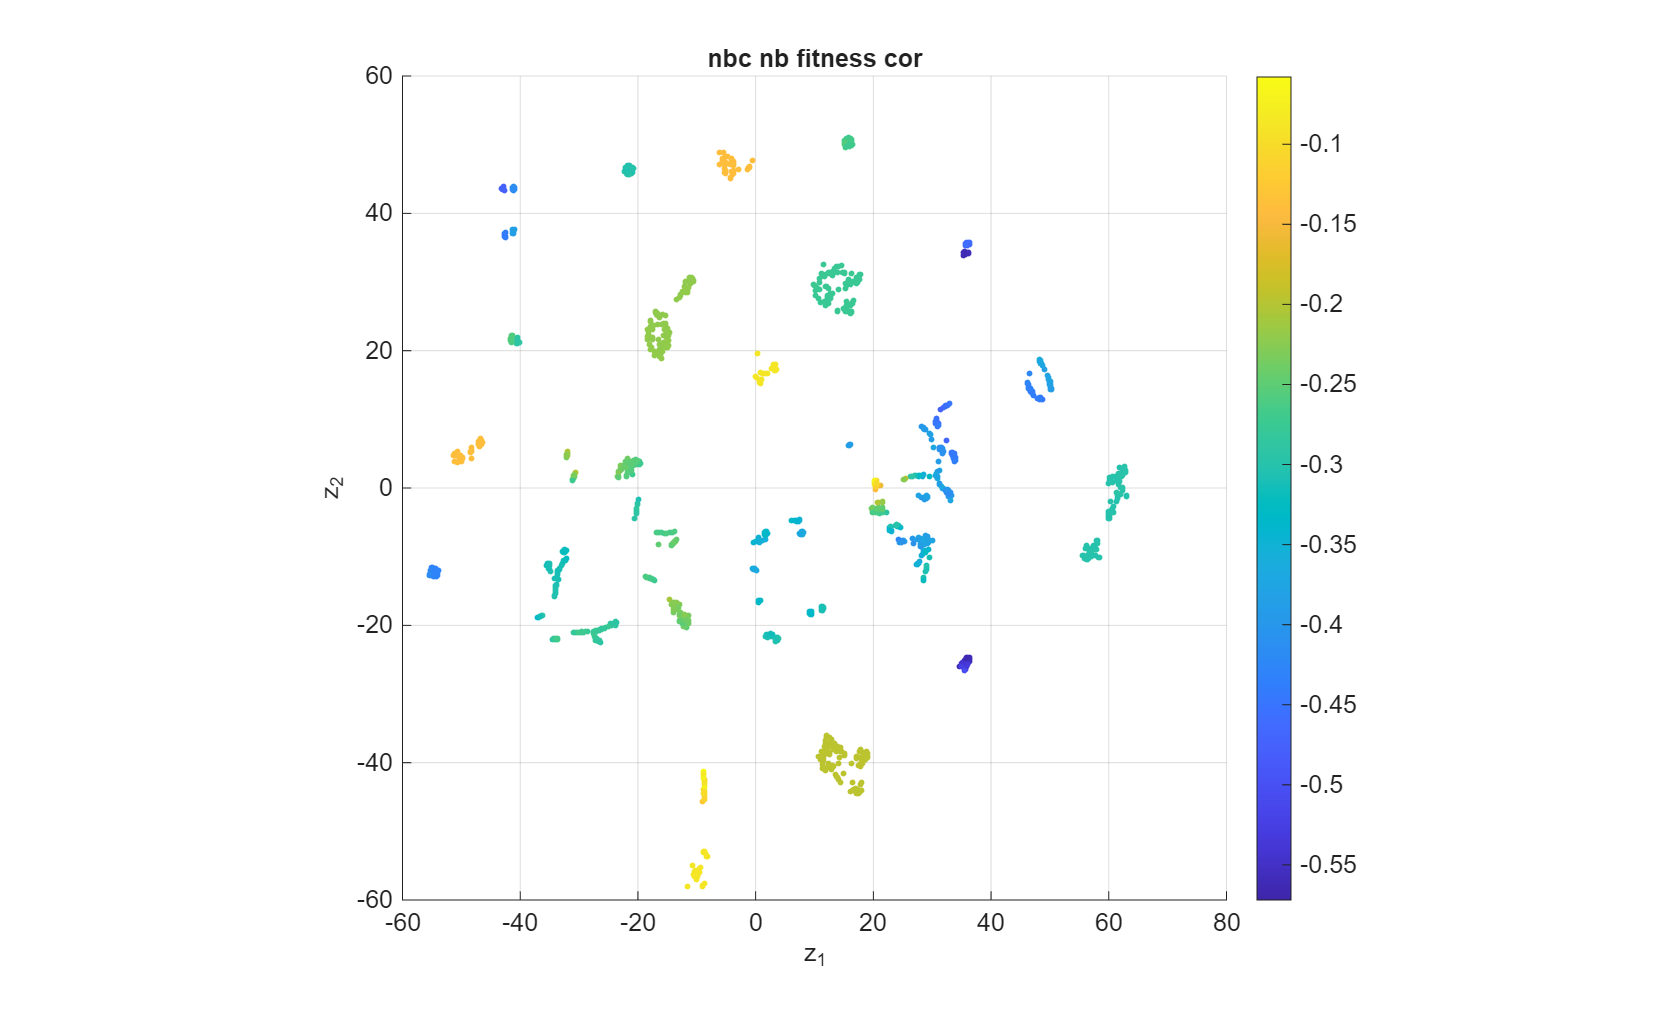
\includegraphics[trim=5.5cm 0.0cm 5.5cm 0.0cm, clip=true, width = 0.47\textwidth]{tsne_nbc_nb_fitness_cor.png}\label{fig:tsne_nbc_nb_fitness_cor}}
    \subfloat[disp\_ratio\_median\_02]{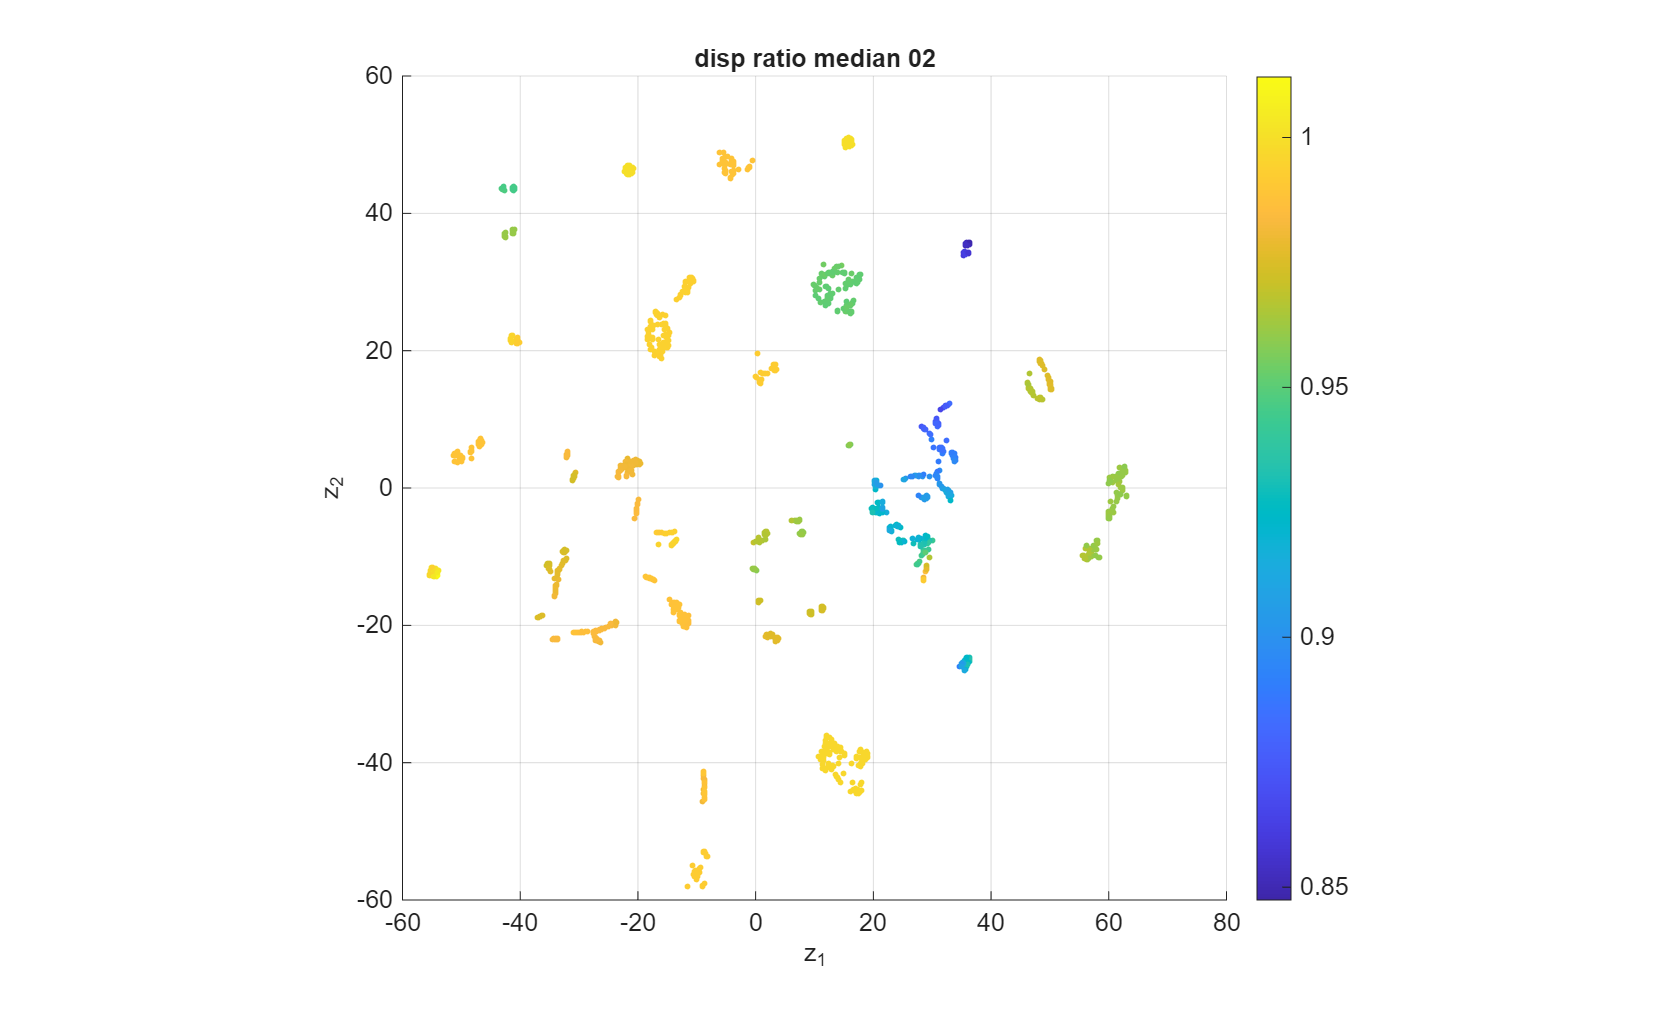
\includegraphics[trim=5.5cm 0.0cm 5.5cm 0.0cm, clip=true, width = 0.47\textwidth]{tsne_disp_ratio_median_02.png}\label{fig:tsne_disp_ratio_median_02}}
	\caption{Feature values of the BBOB and CORNN instances on the instance space, with the colour scale representing the value of the most correlated features with the axes. The CORNN instances are differentiated from the BBOB instances using grey boxes in the first plot.}
	\label{fig:projection_by_features}
\end{figure*}
% -----------------------------------------------------------------------

Second, {\tt ela\_level\_mmce\_qda\_10} fits a linear classifier to distinguish between better and poorer solutions, using the lowest 10\% cost percentile as the decision boundary. The feature quantifies the model's error and can be viewed as a measure of a lack of global structure. 
%Positively correlated with the vertical axis ($z_2$), Figure~\ref{fig:tsne_ela_level_mmce_qda_10} shows that instances beyond the core tend to have higher values of these features, 
Figure~\ref{fig:tsne_ela_level_mmce_qda_10} shows that the CORNN instances are characterised as having high values for this feature, whereas only BBOB instances have low values. An example of a BBOB function with high values is function 16 -- Weierstrass function, distributed across three clusters roughly at $\left[-55,-11\right]$, $\left[-20,45\right]$ and $\left[15,50\right]$, and described as ``Highly rugged and moderately repetitive landscape, where the global optimum is not unique''~\cite{hansen:BBOB}.

Third, {\tt nbc\_nb\_fitness\_cor} describes the correlation between the fitness value and the distance to the nearest-better solutions~\cite{Kerschke2015}, and it is considered a measure of the global-to-local contrast, that is, a lack of difference between local and global optima. Figure~\ref{fig:tsne_nbc_nb_fitness_cor} shows that CORNN instances tend to have higher values of this feature compared to BBOB instances, indicating low contrast. This observation is consistent with~\cite{Malan2025} and aligns with our expectations for the structure of the neural network training task, in which we anticipate finding no global structure and multiple global optima due to symmetry. 

Finally, {\tt disp\_ratio\_median\_02} computes the ratio of the median distance among the 2\% best elements to the overall design distance. Larger values of this ratio indicate multiple funnels that are far apart and can be viewed as a measure of a high degree of multimodality at the global level. In contrast, a landscape with a single funnel, even if highly rugged at a local scale, will have a low value of this ratio. Figure~\ref{fig:tsne_disp_ratio_median_02} shows that the only instances with low values for this feature are BBOB instances. For the CORNN instances, those with medium values (light green) correspond to 1-layer networks. This suggests that deeper networks yield landscapes with a higher degree of global multimodality.

%[ANDRES: TO COMPLETE -- THIS FEATURE ALSO DESCRIBES MULTIMODALITY AND LACK OF GLOBAL STRUCTURE.]

% Secondly, feature {\tt ic\_eps\_max} negatively correlates with the horizontal axis ($z_1$). This feature is one of the information-content features related to the smoothness, ruggedness, and neutrality of the landscape. In particular, {\tt ic\_eps\_max} can be viewed as an indicator of a lack of neutrality (low values of the feature are indicative of high levels of neutrality -- this is explained in~\cite{Malan2009}). Figure \ref{fig:projection_by_features}(d) shows that both of the CORNN clusters are associated with low values for this feature, and the ReLU cluster (bottom right) has lower values than the Tanh cluster, which corresponds with our expectation that the landscapes of ReLU instances would have higher neutrality.

Together, the observations in Figures~\ref{fig:violin_strong_features} and~\ref{fig:projection_by_features} indicate that CORNN instances exhibit features of highly rugged, repetitive functions with multiple global optima, matching the observations on 1-layer CORNN instances~\cite{Malan2025}. However, in~\cite{Malan2025} neutrality was also identified as a distinguishing landscape feature of CORNN instances, but did not emerge as significant in this extended study, including 3- and 5-layer networks. This could indicate that neutral areas decrease in the landscapes of deeper networks, which aligns with the observation from Figure~\ref{fig:tsne_disp_ratio_median_02} that deeper networks have a higher degree of multimodality on a global scale. %However, we were unable to observe features indicative of neutrality. [KATHERINE: ANYTHING TO ADD?]

% ===================================================================
\subsection{Performance analysis}
% ===================================================================
Table~\ref{tab:finds_targets} shows the percentage of instances per set for which one of the four black-box algorithms under analysis, i.e., CMA-ES, PSO, Random Search, and Two-Points DE, finds at least one of the 21 precision targets (see Section~\ref{sec:alg_perf}) -- generally this being the easiest target equal to 10. The final column shows the average across sets.  A first observation is that BBOB instances in these high dimensions are harder to optimise than CORNN instances. 

%[ANDRES - please check new paragraph]
We note that this study differs from the approach used in~\cite{Malan2022} to measure performance, in which performance was reported as the ability of the trained neural network to generalise well. Here, we measure the algorithm's ability to find a set of weights in the network that yields an error of zero within a specified precision on the training dataset. Since there are multiple global optima (and possibly many good local optima), this should be a relatively easy task, as is clear from the fact that even Random Search finds good solutions in most cases. In contrast, for most BBOB instances, algorithms must find a single global optimum or a solution close in value to the optimum, which is much harder.

A second observation from Table~\ref{tab:finds_targets} is that CMA-ES is the best performer at finding targets on these instances, followed by two-points DE, whereas PSO performs at least as poorly as Random Search. CORNN instances with the ReLU activation function are harder to optimise for PSO and Random Search than those with the Tanh activation function for the 3- and 5-layer networks. Note that ReLU maps all negative inputs to zero, thereby introducing neutrality in the network's output and the associated error landscape. Neutrality implies a lack of information in the landscape and may explain the performance difference between ReLU and Tanh instances. 
%[KATHERINE: IS MY THEORY OF THE SIMILAR NEUTRALITY RUINING PBEST AND GBEST INFORMATION LOGICAL?].
%
% -----------------------------------------------------------------------
%[ANDRES - I have taken out the entries for the test sets. It makes sense to analyse the test error landscape, but it does not make sense to optimise the test landscape]
\begin{table}[!t]
    \caption{Percentage of instances per set for which a black-box algorithm finds at least one of the precision targets. On average, BBOB instances are harder than CORNN instances, and CORNN instances with ReLU activation function are harder than those with Tanh activation function.}
    \label{tab:finds_targets}
    \footnotesize
    \begin{tabular}{lrrrrr}
        \toprule
                                               & CMA-ES   & PSO   & Random Search & Two-Points DE & Average \\
        \midrule
        BBOB\textsubscript{D=41}               & 47\%  & 4\%   & 4\%          & 37\%        & 23\%    \\
        BBOB\textsubscript{D=261}              & 32\%  & 4\%   & 4\%          & 4\%         & 11\%    \\
        BBOB\textsubscript{D=481}              & 32\%  & 4\%   & 4\%          & 4\%         & 11\%    \\
        CORNN\textsubscript{Net1, ReLU%, Train
        } & 100\% & 100\% & 100\%        & 100\%       & 100\%   \\
        %CORNN\textsubscript{Net1, ReLU, Test}  & 100\% & 100\% & 100\%        & 100\%       & 100\%   \\
        CORNN\textsubscript{Net3, ReLU%, Train
        } & 100\% & 0\%   & 35\%         & 100\%       & 59\%    \\
        %CORNN\textsubscript{Net3, ReLU, Test}  & 100\% & 2\%   & 37\%         & 100\%       & 60\%    \\
        CORNN\textsubscript{Net5, ReLU%, Train
        } & 100\% & 9\%   & 78\%         & 100\%       & 72\%    \\
        %CORNN\textsubscript{Net5, ReLU, Test}  & 100\% & 6\%   & 89\%         & 100\%       & 74\%    \\
        CORNN\textsubscript{Net1, Tanh%, Train
        } & 100\% & 100\% & 100\%        & 100\%       & 100\%   \\
        %CORNN\textsubscript{Net1, Tanh, Test}  & 100\% & 100\% & 100\%        & 100\%       & 100\%   \\
        CORNN\textsubscript{Net3, Tanh%, Train
        } & 100\% & 100\% & 100\%        & 100\%       & 100\%   \\
        %CORNN\textsubscript{Net3, Tanh, Test}  & 100\% & 100\% & 100\%        & 100\%       & 100\%   \\
        CORNN\textsubscript{Net5, Tanh%, Train
        } & 100\% & 100\% & 100\%        & 100\%       & 100\%   \\
        %CORNN\textsubscript{Net5, Tanh, Test}  & 100\% & 100\% & 100\%        & 100\%       & 100\%  \\
        \bottomrule
    \end{tabular}
\end{table}
% -----------------------------------------------------------------------
%
% -----------------------------------------------------------------------

Figure~\ref{fig:distribution_performance} illustrates the performance of the different algorithms across the instance space, with colour representing the AUC for each instance. A higher value represents easier problems, for which more targets are reached, whereas a lower value represents problems for which fewer targets are reached. For CMA-ES, Figure~\ref{fig:distribution_performance_CMA} shows that the CORNN instances generally have high values of AUC, resulting in all targets being reached, whereas this is not the case for all BBOB functions, for which, in a few instances, a few targets are found, and more often no target is found. For PSO, shown in Figure~\ref{fig:distribution_performance_PSO}, and Random Search, shown in Figure~\ref{fig:distribution_performance_RandomSearch}, we observe that instances have generally low values of AUC, with a few instances having medium-low values, representing that a few targets were reached, with the easier functions being CORNN functions with Tanh activation. Finally, for Two-Points DE, Figure~\ref{fig:distribution_performance_TwoPointsDE} shows that, for most CORNN instances, a medium AUC value is obtained, indicating that some targets are reached but generally underperforming CMA-ES.

% -----------------------------------------------------------------------
%
% -----------------------------------------------------------------------
\begin{figure*}[!t]
    \centering
    \subfloat[CMA-ES]{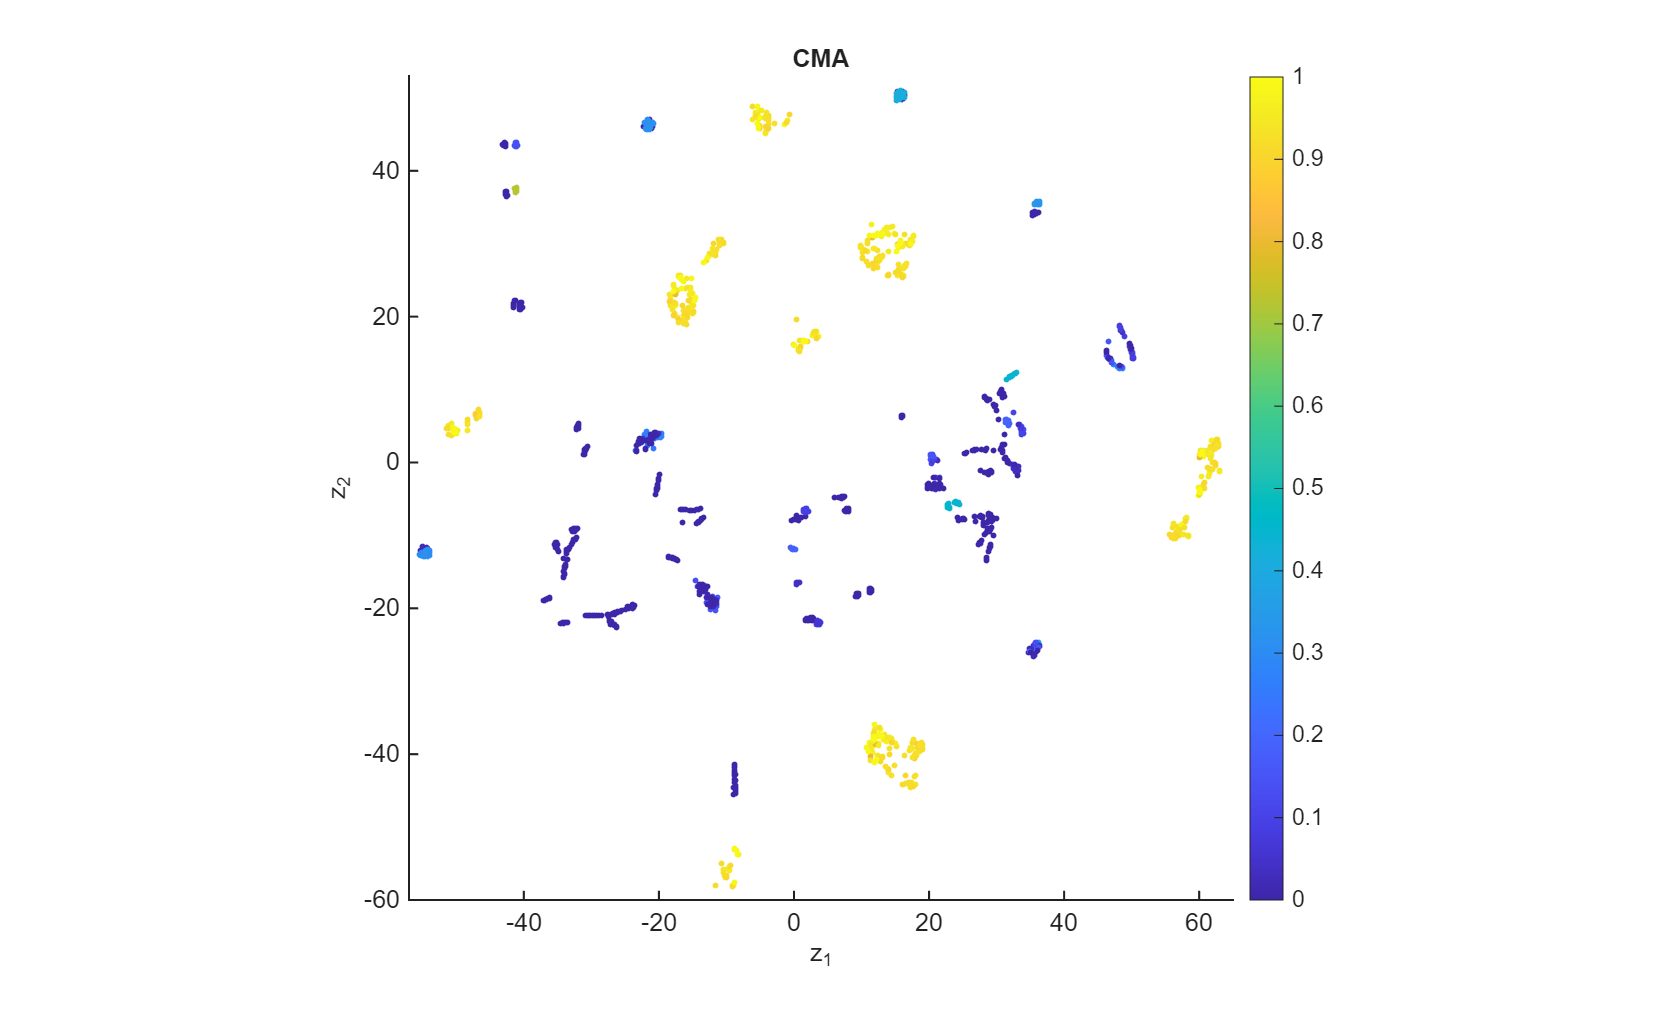
\includegraphics[trim=5.5cm 0.0cm 5.5cm 0.0cm, clip=true, width = 0.47\textwidth]{distribution_performance_CMA.png}\label{fig:distribution_performance_CMA}}
    \subfloat[PSO]{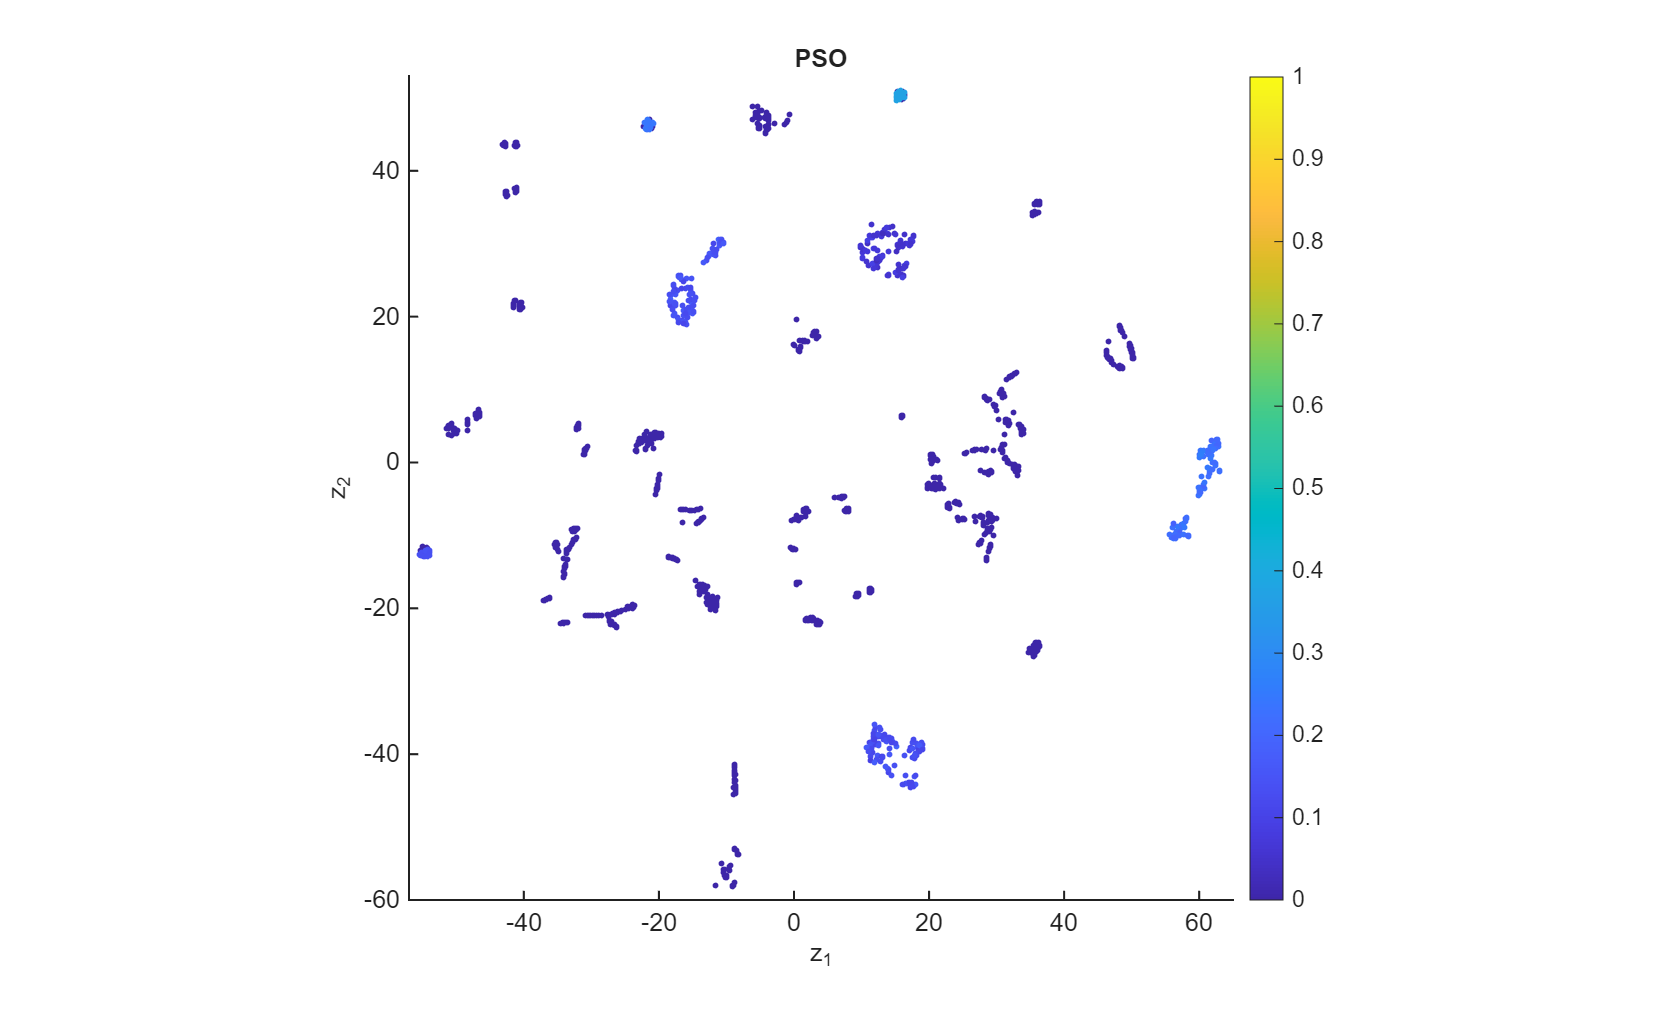
\includegraphics[trim=5.5cm 0.0cm 5.5cm 0.0cm, clip=true, width = 0.47\textwidth]{distribution_performance_PSO.png}\label{fig:distribution_performance_PSO}}\\
    \subfloat[Random Search]{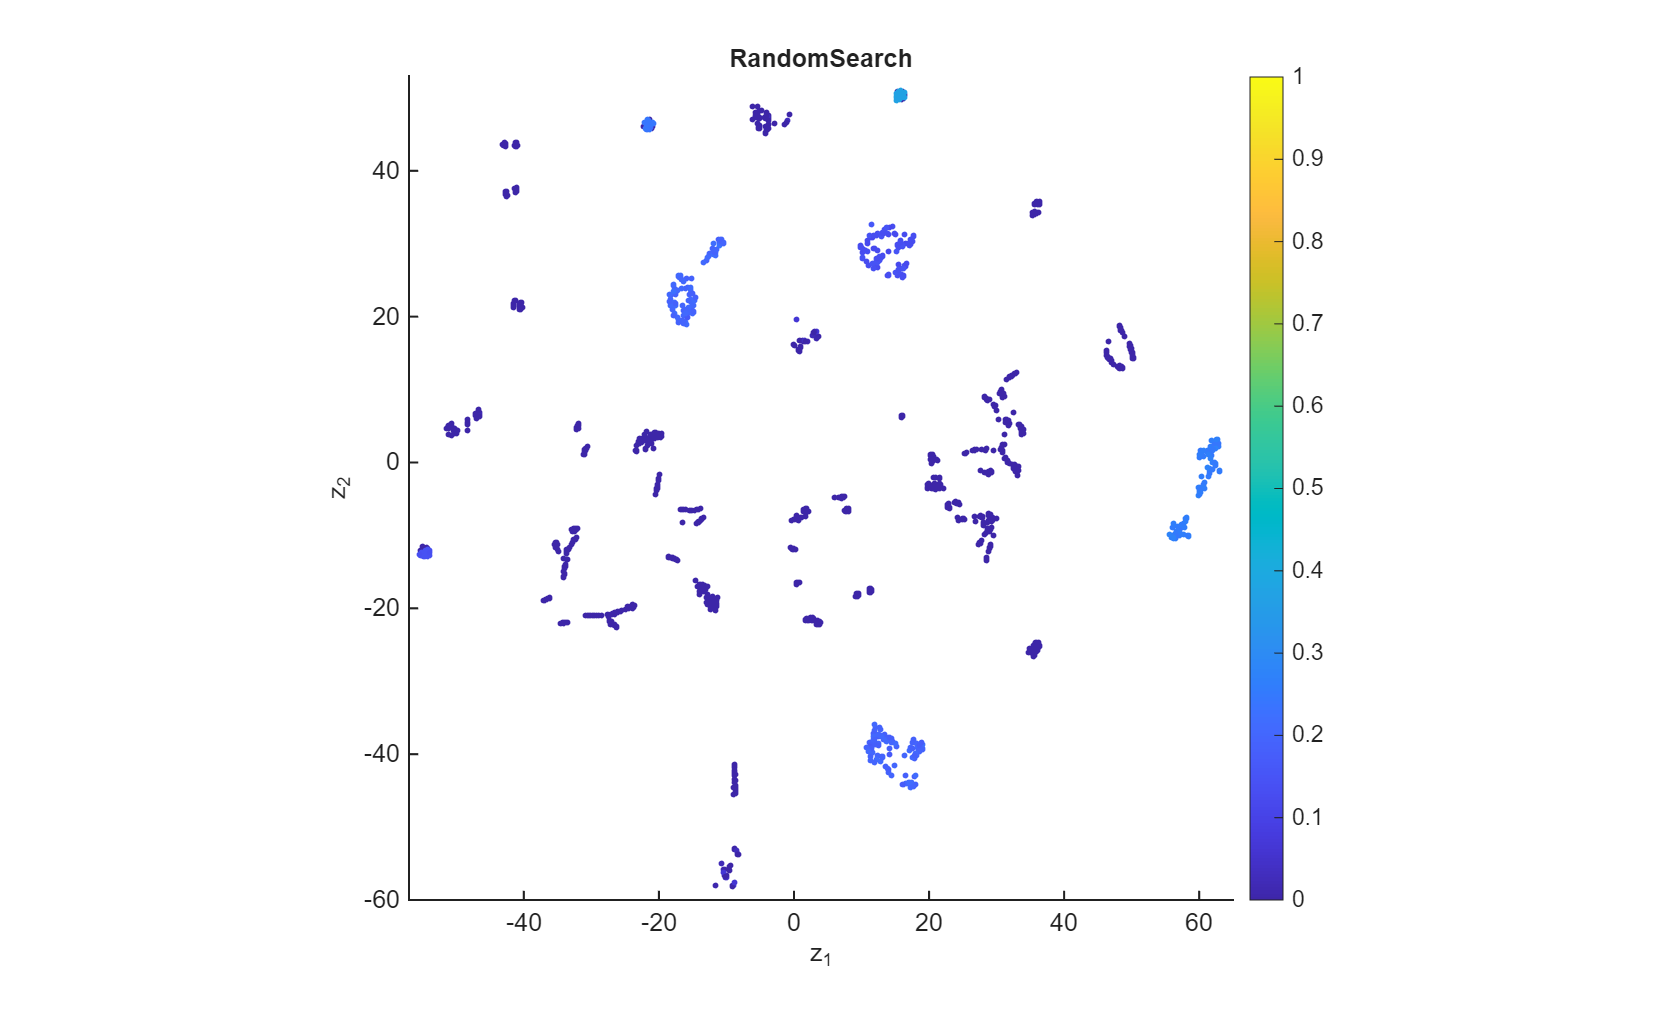
\includegraphics[trim=5.5cm 0.0cm 5.5cm 0.0cm, clip=true, width = 0.47\textwidth]{distribution_performance_RandomSearch.png}\label{fig:distribution_performance_RandomSearch}}
    \subfloat[Two-Points DE]{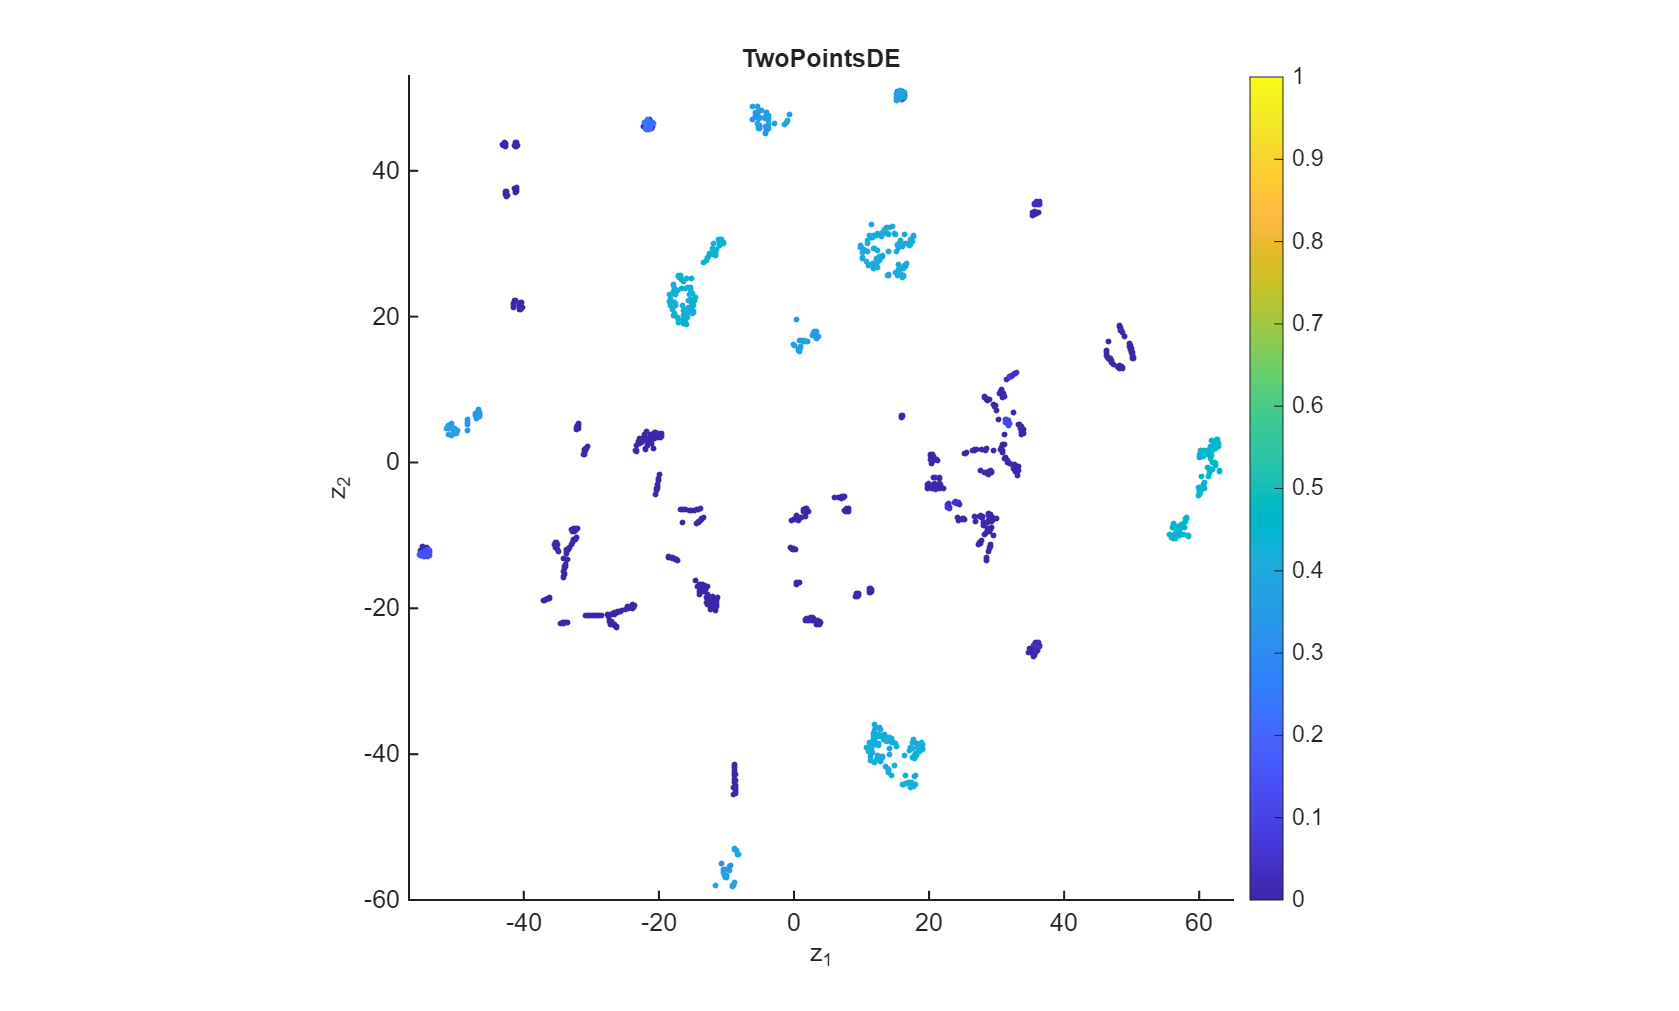
\includegraphics[trim=5.5cm 0.0cm 5.5cm 0.0cm, clip=true, width = 0.47\textwidth]{distribution_performance_TwoPointsDE.png}\label{fig:distribution_performance_TwoPointsDE}}
	\caption{Performance values, measured as the area under the curve (AUC) of the empirical cumulative probability function (ECDF), for the four evaluated algorithms across the instance space. Lighter colour (yellow) represents a high AUC, indicating that a high number of targets were reached, whereas a darker colour (blue) represents a low AUC, indicating that a low number of targets were reached.}
	\label{fig:distribution_performance}
\end{figure*}
% -----------------------------------------------------------------------

Figure~\ref{fig:footprint} illustrates the footprints of each algorithm, with the acceptability criteria being to reach at least one target. Surprisingly, the instances within the `core' are generally harder than those in the periphery, meaning that multi-modal instances have local optima that are acceptable. These results are further quantified in Table~\ref{tab:footprint_analysis}, which shows the normalised area ($\alpha$), density ($d$), and purity ($p$) of the footprints obtained through TRACE\textsuperscript{3}, which tends to be conservative. Both acceptable ($A$) and best ($B$) performance footprints are shown, with acceptable performance defined as AUC > 0 and best performance as the highest AUC. Under these criteria, CMA-ES outperforms all other algorithms, but is relatively weak, covering only 16.8\% of the space. All footprints are highly dense, except for the Two-Points DE best footprint, where, despite its small size, it retains a relatively high level of contradictions.

% -----------------------------------------------------------------------
\begin{figure*}[!t]
    \centering
    \subfloat[CMA-ES]{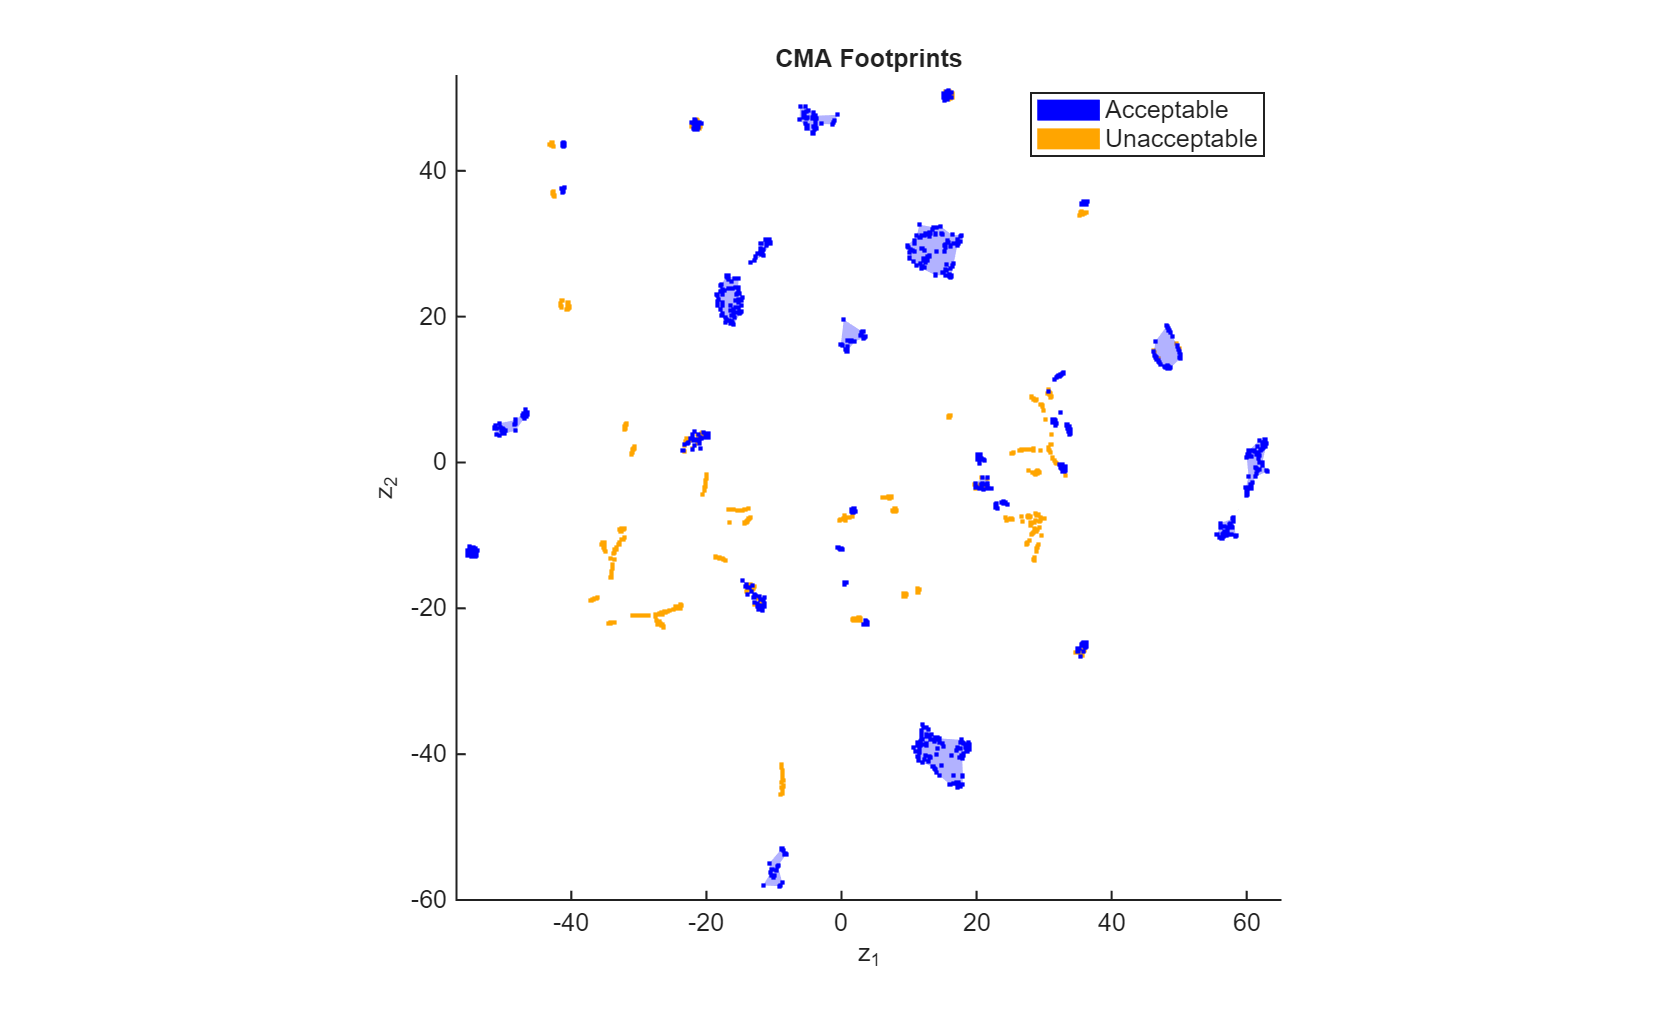
\includegraphics[trim=6.0cm 0.0cm 6.5cm 0.0cm, clip=true, width = 0.47\textwidth]{Figures/footprint_CMA_eps0.png}}
    \subfloat[PSO]{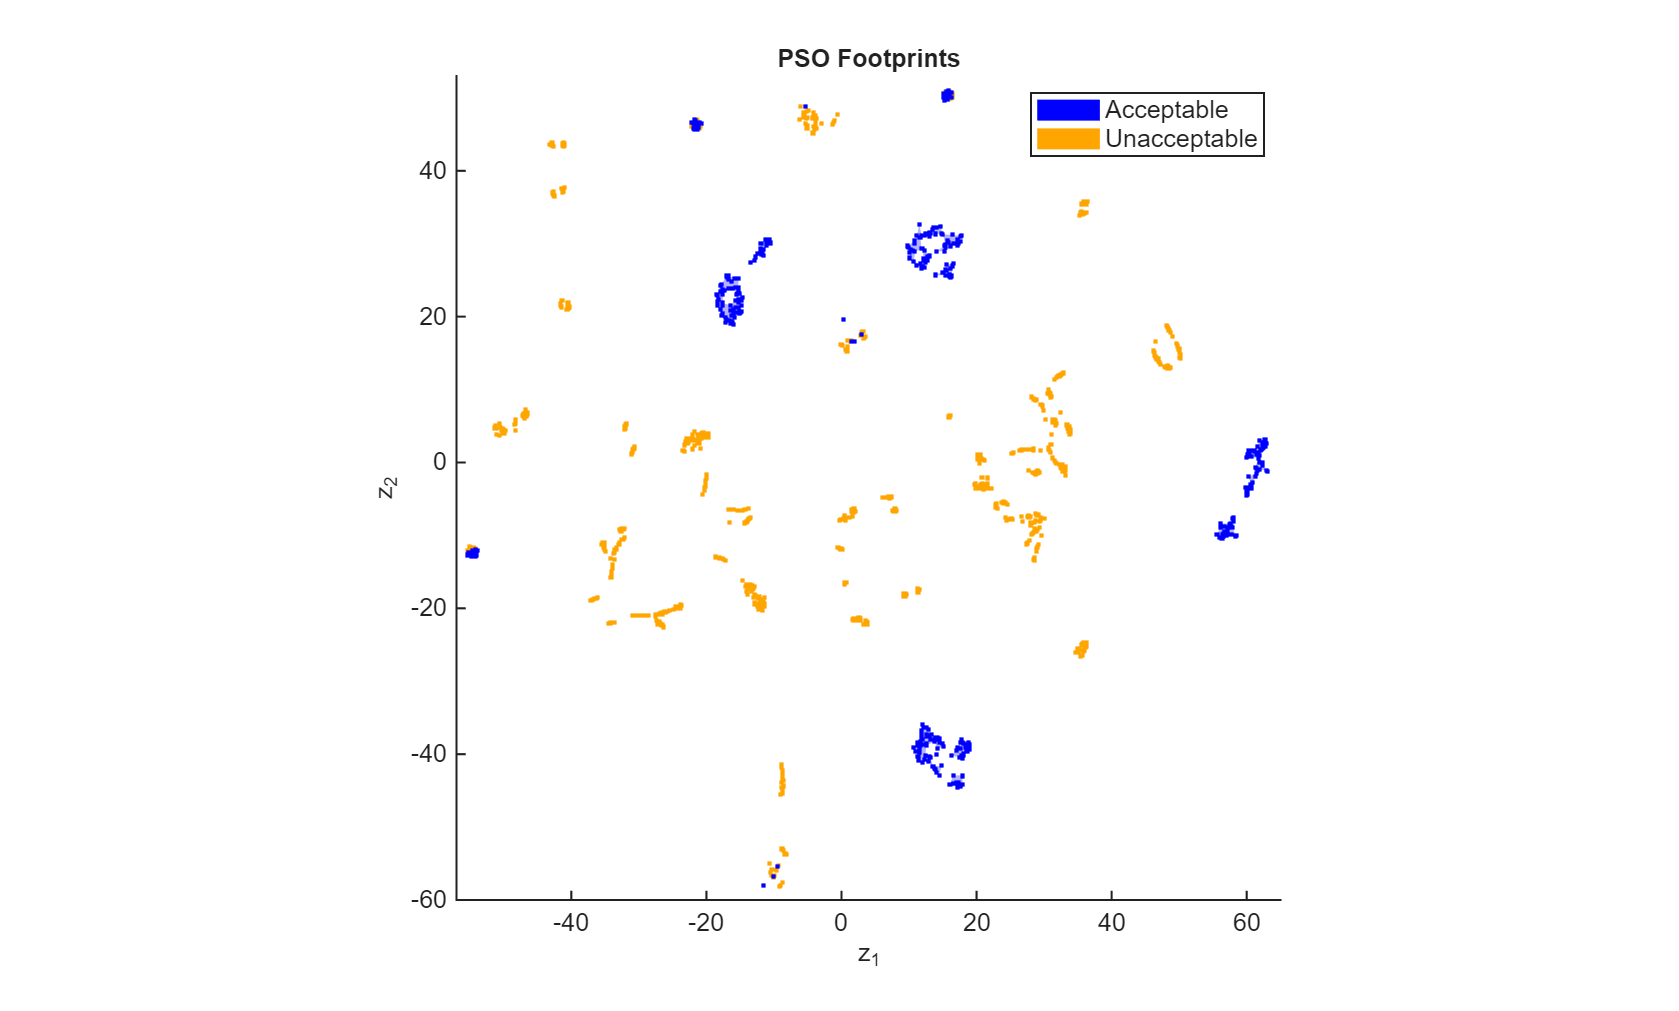
\includegraphics[trim=6.0cm 0.0cm 6.5cm 0.0cm, clip=true, width = 0.47\textwidth]{Figures/footprint_PSO_eps0.png}}\\
    \subfloat[Random Search]{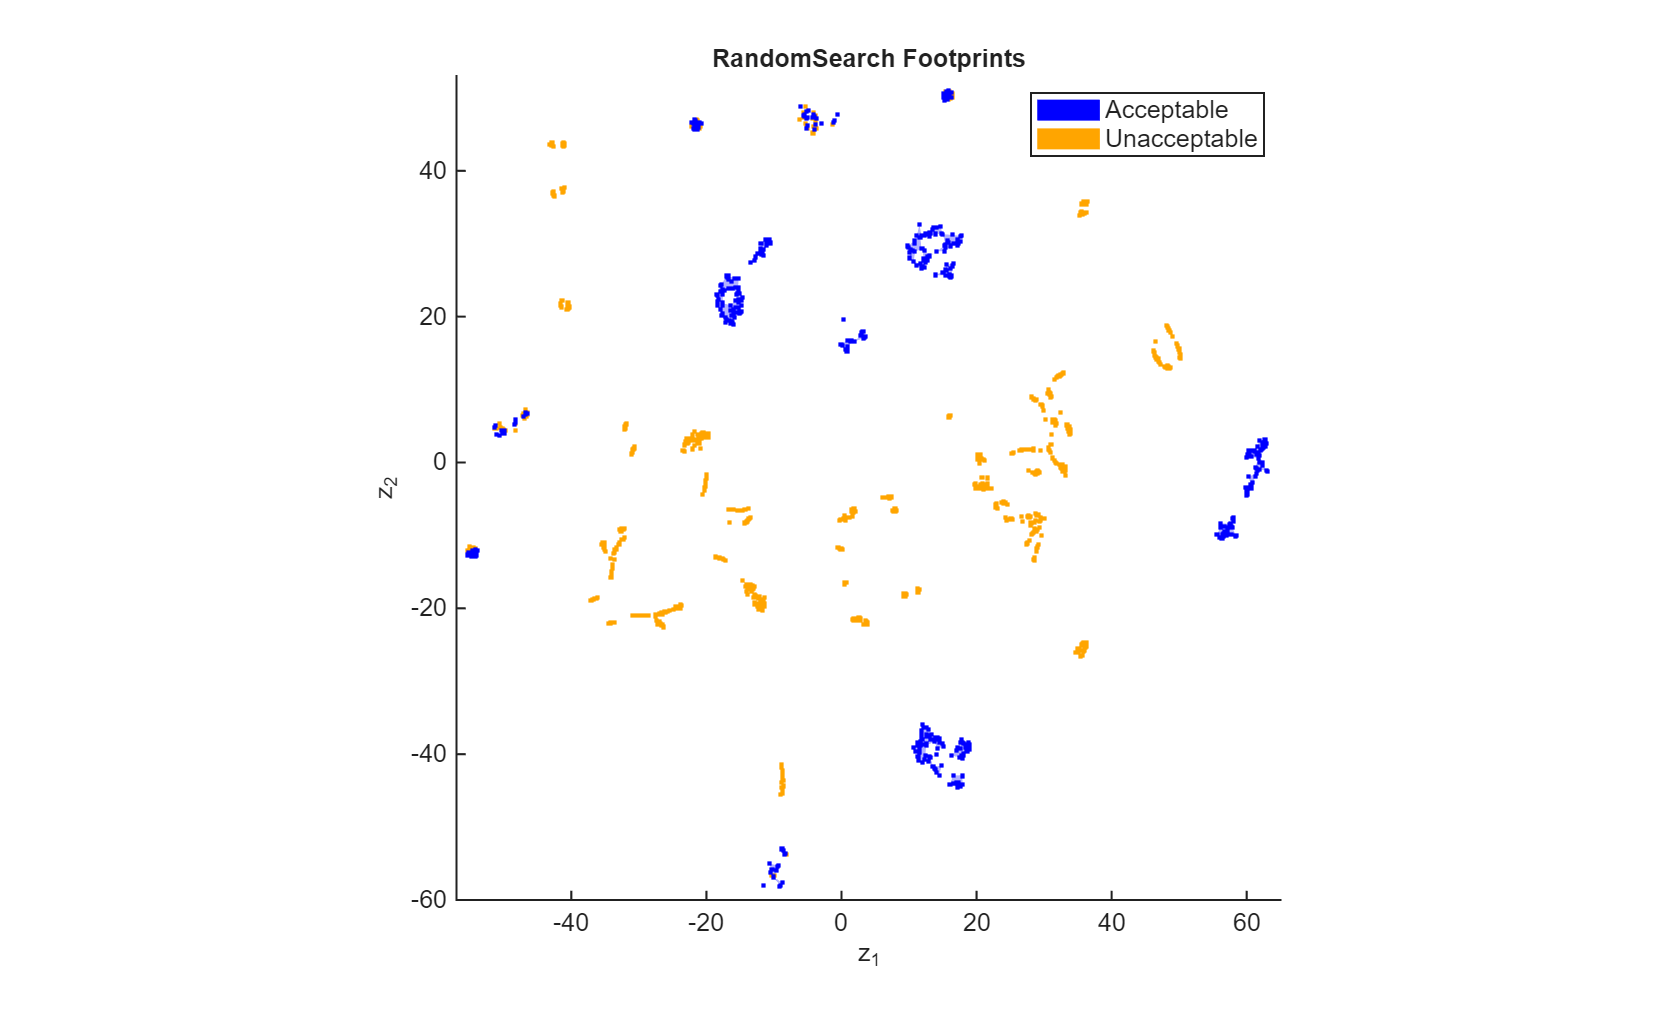
\includegraphics[trim=6.0cm 0.0cm 6.5cm 0.0cm, clip=true, width = 0.47\textwidth]{Figures/footprint_RandomSearch_eps0.png}}
    \subfloat[Two-Points DE]{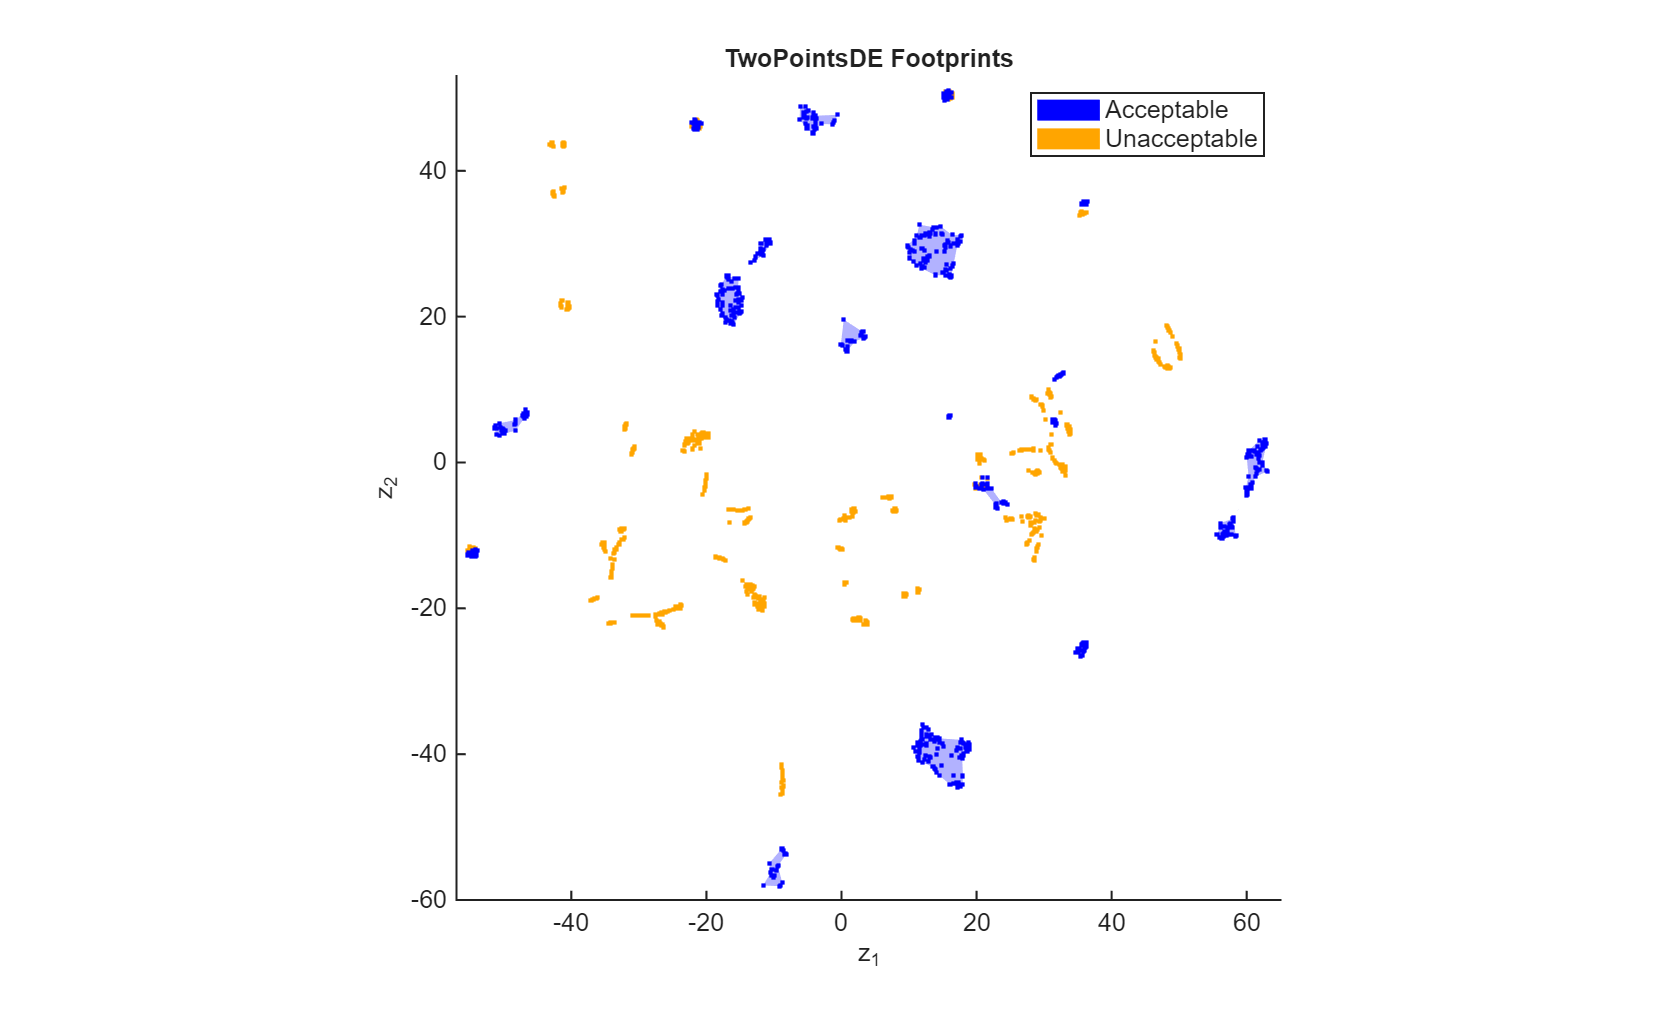
\includegraphics[trim=6.0cm 0.0cm 6.5cm 0.0cm, clip=true, width = 0.47\textwidth]{Figures/footprint_TwoPointsDE_eps0.png}}
	\caption{Footprints for the four algorithms under analysis, with acceptable performance defined as finding at least one target. The figure demonstrates that instances at the `core' are generally harder than instances in the periphery, which include the CORNN instances and others with high modality and poor global structure.}
	\label{fig:footprint}
\end{figure*}
% -----------------------------------------------------------------------
%
% -----------------------------------------------------------------------
\begin{table}[!t]
    \centering
    \caption{Footprint analysis for CMA-ES, PSO, Random Search, and Two-Points DE, with acceptable performance being defined as having an AUC greater than zero, and best performance is defined as having the highest AUC that is not zero. Under these criteria, CMA-ES outperforms all other algorithms.}
    \label{tab:footprint_analysis}
    \footnotesize
    \begin{tabular}{lcccccc}
        \toprule
        & $\alpha_{N,A}$ & $d_{N,A}$ & $p_{A}$ &
          $\alpha_{N,B}$ & $d_{N,B}$ & $p_{B}$ \\
        % \midrule
        % \multicolumn{7}{c}{Actual} \\
        \midrule
        CMA-ES          & 17.0\% & 287.5\% & 96.6\% & 16.8\% & 283.2\%  & 97.8\% \\
        PSO          & 5.9\%  & 444.5\% & 98.7\% & 0.0\%  & 0.0\%    & 0.0\%  \\
        Random Search & 6.5\%  & 528.8\% & 95.3\% & 0.0\%  & 0.0\%    & 0.0\%  \\
        Two-Points DE  & 15.8\% & 284.1\% & 97.3\% & 0.2\%  & 1143.1\% & 70.8\%\\
        % \midrule
        % \multicolumn{7}{c}{Predicted} \\
        % \midrule
        % CMA          & 22.8\% & 271.1\% & 99.6\%  & 18.8\% & 309.5\% & 98.4\% \\
        % PSO          & 34.2\% & 112.3\% & 99.2\%  & 0.8\%  & 750.6\% & 61.5\% \\
        % RandomSearch & 23.4\% & 197.8\% & 100.0\% & 0.8\%  & 465.7\% & 63.5\% \\
        % TwoPointsDE  & 40.0\% & 140.1\% & 99.6\%  & 25.5\% & 63.5\%  & 62.5\%  \\
        \bottomrule
    \end{tabular}
\end{table}
% -----------------------------------------------------------------------

% ===================================================================
\subsection{Discussion}\label{sec:discussion}
% ===================================================================
From the analysis of the instance space, the individual features, and the performance of algorithms, we deduce the following.

Firstly, the clear separation between the BBOB and CORNN instances in the 2$D$ instance space across all dimensions indicates that the features of the landscapes of the CORNN instances differ from those of the BBOB functions. Most of the BBOB functions form a central cluster in the instance space, with only a few functions interspersed between the CORNN instances toward the edges of the map. Further analysis of the ELA features shows that the BBOB functions in the central cluster of the instance space are characterised by strong global structure, with a single or a few funnels and large differences between local and global optima. In contrast, the CORNN suite instances lack global structure and exhibit many similar local and global optima. Neutrality did not emerge as a distinguishing landscape feature in the 3- and 5-layer CORNN suite instances as it did in the 1-layer instances~\cite{Malan2025}.

The instance space also reveals that the CORNN instances form distinct clusters based on the activation function (ReLU or Tanh) and the network dimension (number of layers), but not on the underlying regression function. This suggests that the features of neural network error landscapes are more strongly influenced by the choice of activation function and network size than by the machine learning task itself. An interesting observation was that the ReLU training and testing instances formed distinct clusters (not observed for Tanh instances) for the 3- and 5-layer networks (not the 1-layer networks), and the distance between clusters was significantly larger for the 5-layer networks. This indicates that the features differ between the training and testing error landscapes: they `look' different, so finding good solutions in the training landscape does not necessarily translate to good solutions in the testing landscape. This discrepancy could negatively affect the ability of larger ReLU networks to generalise to unseen data.

Performance analysis in the instance space showed that all algorithms struggled with problems characterised by strong global structure, with single or a few funnels and large differences between local and global optima. In contrast, algorithms were more likely to find good solutions when the landscapes were highly rugged on a global scale, with smaller differences between local and global optima. CMA-ES was the best-performing algorithm of the four over the full set of BBOB and CORNN instances.

In the original CORNN suite paper~\cite{Malan2022}, the performance of the best black-box algorithm (of the four also considered in this study) was compared
with the performance of Adam. Based on mean squared error (MSE), Adam outperformed the best black-box algorithm on all but a few of the CORNN instances. Bearing this in mind, although the CORNN instances were regarded as ``relatively easy" for the black-box algorithms compared with the BBOB instances in this study, this performance would be regarded as inferior in comparison with Adam for most of the CORNN instances. The exploitative behaviour of gradient-based approaches appears beneficial on ill-conditioned landscapes with many reasonably good solutions.
% ===================================================================
\section{Conclusions}\label{sec:conclusion}
% ===================================================================
In this paper, we performed an instance space analysis of 1-, 3-, and 5-layer instances from the CORNN suite, corresponding to search spaces with 41, 261, and 482 continuous-valued decision variables. We included BBOB instances with the same number of dimensions, enabling us to compare the CORNN suite against BBOB with respect to ELA features and black-box algorithm performance. 

Unlike most BBOB functions, we demonstrate that CORNN instances exhibit weak or no global structure, with multiple optima and small differences between local and global optima. These ill-conditioned landscapes were easier to optimise for black-box algorithms, an unexpected result that can be understood in light of the abundance of reasonably good solutions. The key differentiators between CORNN instances were the activation function (ReLU or Tanh) and the dimension of the search space, and, surprisingly, not the underlying regression problem. The neutrality of the error landscape of CORNN instances, previously observed in 1-layer instances, did not hold for deeper networks -- another surprising result. 

In future work, we plan to investigate the effect of the search space bounds of the CORNN instances on the analysis. In this study, the weight space sample for ELA was bound to $\left[-5,5\right]$. Unlike the BBOB functions, however, the weight space is unbounded in practice. It would be interesting to investigate the effect that extending these bounds has on the ELA features of CORNN instances.

In the original CORNN paper~\cite{Malan2022}, black-box algorithms were benchmarked against the gradient-based algorithm, Adam. Although Adam generally performed better, the black-box algorithms outperformed Adam on a limited set of regression problem instances. Future work could include performance data to identify footprints of Adam in the instance space. If viewed alongside the black-box algorithm footprints, this could help us identify which instances are better suited to gradient-based and black-box approaches and analyse why (by analysing instance features).

% ===================================================================
\begin{acks}
    The \grantsponsor{ARCIC}{Australian Research Council}{https://www.arc.gov.au/} has partially funded this work through grant No.:~\grantnum[]{ARCIC}{IC200100009}. M.A. Muñoz is also with the ARC Training Centre in Optimisation Technologies, Integrated Methodologies and Applications (OPTIMA). This research was supported by The University of Melbourne’s Research Computing Services and the Petascale Campus Initiative.
    
    During the preparation of the experimental work and this manuscript, M.A. Muñoz used professional versions of PyCharm 2025.2 [\url{https://www.jetbrains.com/pycharm/}], MATLAB R2025a [\url{https://au.mathworks.com/products/matlab.html}], and Grammarly [\url{https://app.grammarly.com/}]. PyCharm AI Assistant was used to improve the stability of the Python scripts developed by generating exception handling and optimising memory management. MATLAB Copilot was used to identify bugs and improve code performance by generating vectorised code to replace iterating sections. Grammarly was used to check expression and grammar, and rephrasing, after which the author reviewed and edited the content as needed. The author takes full responsibility for the code and content of the published article.
\end{acks}
% ===================================================================
%\bibliographystyle{ACM-Reference-Format}
\bibliographystyle{ACM-Reference-Format}
\bibliography{reflist}
% ===================================================================
% \appendix
% \section{Some Appendix}
% ===================================================================
\end{document}
% ===================================================================
